\section{Защита данных в распределенных системах}
\subsection{Распределенные вычислительные среды}
Распределённая обработка данных - методика выполнения прикладных программ группой систем.
При этом пользователь получает возможность работать с сетевыми службами и прикладными процессами,
расположенными в нескольких взаимосвязанных абонентских системах. \autocite{Sergeeva}

\paragraph{
    Распределенная обработка информации в среде клиент-сервер.
    Концепция распределенной вычислительной среды Distributed Computing Environment (DCE).
    Распределенные базы данных в сетях ЭВМ
} ~\\

Компьютер (или программу), управляющий ресурсом, называют сервером этого ресурса (файлсервер, сервер базы данных,
вычислительный сервер...). Клиент и сервер какого-либо ресурса могут находиться как в рамках одной вычислительной системы,
так и на различных компьютерах, связанных сетью. Основной принцип технологии "клиент-сервер" заключается в разделении
функций приложения на три группы \autocite{4studClntSrv}:
\begin{itemize}
    \item ввод и отображение данных (взаимодействие с пользователем);
    \item прикладные функции, характерные для данной предметной области;
    \item функции управления ресурсами (файловой системой, базой данных и т.д.)
\end{itemize}

Поэтому, в любом приложении можно выделить следующие компоненты:
\begin{itemize}
    \item компонент представления данных
    \item прикладной компонент
    \item компонент управления ресурсом
\end{itemize}

Связь между компонентами осуществляется по определенным правилам, которые называют "протокол взаимодействия".
Каждый из компонентов приложения при этом может работать на выделенном сервере (узле) или разделять ресурсы сервера
с другими компонентами приложения. В связи с этим можно выделить следующие модели приложений:
\begin{itemize}
    \item двухзвенная модель (модель «клиент-сервер»)
    \item трехзвенная модель (модель сервера приложений)
    \item многозвенная модель
\end{itemize}

\textbf{Двухзвенная модель} позволяет распределить различным образом три компонента приложения между двумя узлами 
\textbf{Трехзвенная модель} предполагает выделение для каждого из трех компонентов приложения свой сервер \autocite{4studClntSrv}.
\textbf{Многозвенная модель} позволяет отдельным компонентам использовать ресурсы нескольких серверов, например,
распределенные базы данных. Компанией Gartner Group, специализирующейся в области исследования информационных технологий,
предложена следующая классификация двухзвенных моделей взаимодействия клиент-сервер \autocite(bmstu)

\begin{figure}[h!]
    \centering
    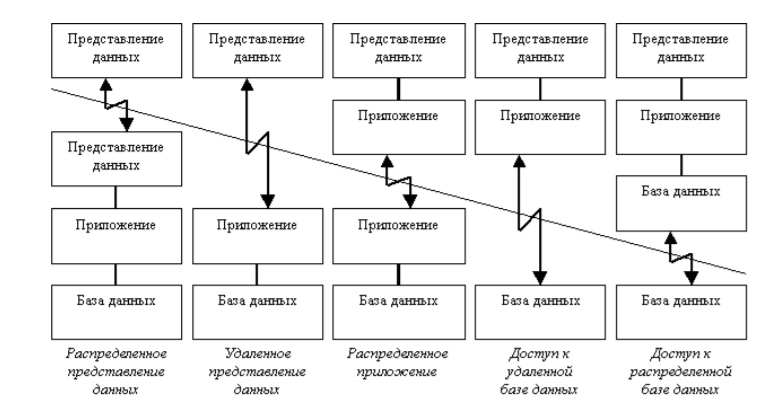
\includegraphics[width=0.8\textwidth]{assets/dce.jpg}
    \caption{Классификация двухзвенных моделей}
\end{figure}

\subparagraph{Двухзвенная структура}~\\
В любой сети, построенной на современных сетевых технологиях, присутствуют элементы
клиент-серверного взаимодействия,часто на основе двухзвенной архитектуры.

\begin{figure}[h!]
    \centering
    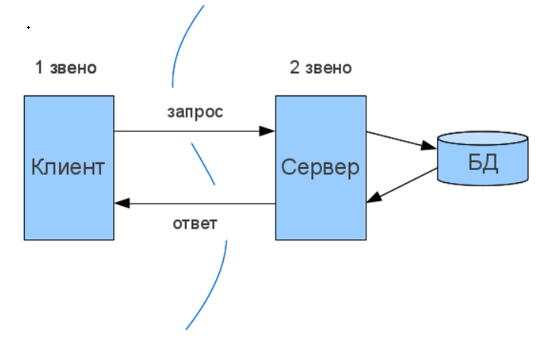
\includegraphics[width=0.8\textwidth]{assets/662}
    \caption{Двухзвенная архитектура}
\end{figure}

Двухзвенная архитектура используется в клиент-серверных системах, где сервер отвечает
на клиентские запросы напрямую и в полном объеме, при этом используя только
собственные ресурсы. Т.е. сервер не вызывает сторонние сетевые приложения и не
обращается к сторонним ресурсам для выполнения какой-либо части запроса.

\begin{figure}[h!]
    \centering
    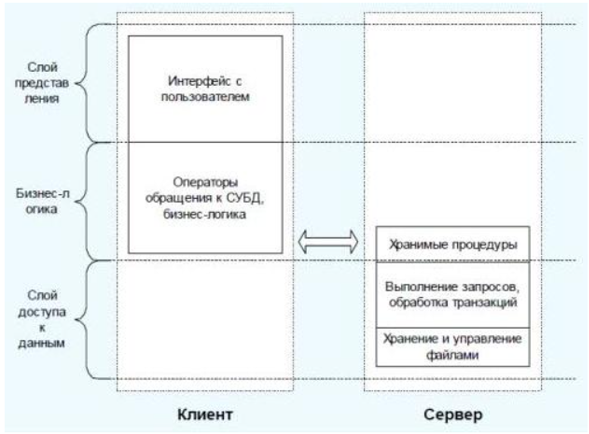
\includegraphics[width=0.8\textwidth]{assets/663}
    \caption{Типичный пример двухзвенной модели}
\end{figure}~\\

Клиентская программа работает с данными через запросы к серверному ПО. Базовые
функции приложения разделены между клиентом и сервером.

Плюсы:
\begin{itemize}
    \item Отсутствие дублирования кода программы-сервера программами-клиентами.
    \item Так как все вычисления выполняются на сервере, то требования к компьютерам, на которых установлен клиент, снижаются.
    \item Все данные хранятся на сервере, который, как правило, защищён гораздо лучше большинства клиентов. На сервере проще обеспечить контроль полномочий, чтобы разрешать доступ к данным только клиентам с соответствующими правами доступа.
    \item Позволяет объединить различные клиенты. Использовать ресурсы одного сервера часто могут клиенты с разными аппаратными платформами, операционными системами и т. п.
    \item Позволяет разгрузить сети за счёт того, что между сервером и клиентом передаются небольшие порции данных.
\end{itemize}

Минусы:
\begin{itemize}
    \item 	Бизнес логика приложений осталась в клиентском ПО. При любом изменении алгоритмов, надо обновлять пользовательское ПО на каждом клиенте.
    \item Высокие требования к пропускной способности коммуникационных каналов с сервером, что препятствует использование клиентских станций иначе как в локальной сети.
    \item Слабая защита данных от взлома, в особенности от недобросовестных пользователей системы.
    \item Высокая сложность администрирования и настройки рабочих мест пользователей системы.
    \item Необходимость использовать мощные ПК на клиентских местах.
    \item Высокая сложность разработки системы из-за необходимости выполнять бизнес-логику и обеспечивать пользовательский интерфейс в одной программе.
\end{itemize}

\subparagraph{Трехзвенная архитектура}~\\

Еще одна тенденция в клиент-серверных технологиях связана со все большим
использованием распределенных вычислений. Они реализуются на основе модели сервера
приложений, где сетевое приложение разделено на две и более частей, каждая из которых
может выполняться на отдельном компьютере. Выделенные части приложения
взаимодействуют друг с другом, обмениваясь сообщениями в заранее согласованном
формате. В этом случае двухзвенная клиент-серверная архитектура становится
трехзвенной.  На этой архитектуре построены большинство современных web-приложений.~\\

\begin{figure}[h!]
    \centering
    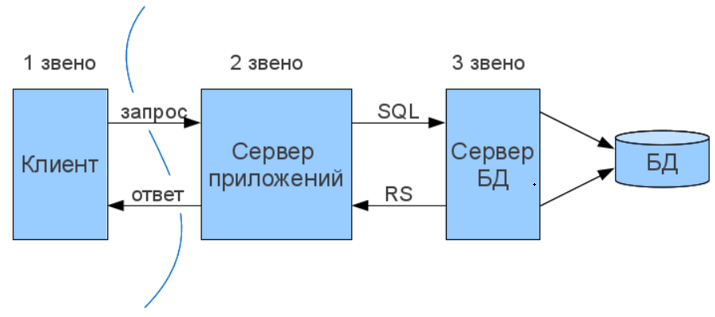
\includegraphics[width=0.8\textwidth]{assets/664}
    \caption{Трехзвенная архитектура}
\end{figure}

Основным ее отличием от предыдущей архитектуры является физическое разделение
программ, отвечающих за хранение данных (СУБД) от программ эти данные
обрабатывающих. Такое разделение программных компонент позволяет оптимизировать
нагрузки как на сетевое, так и на вычислительное оборудование комплекса.~\\

\begin{figure}[h!]
    \centering
    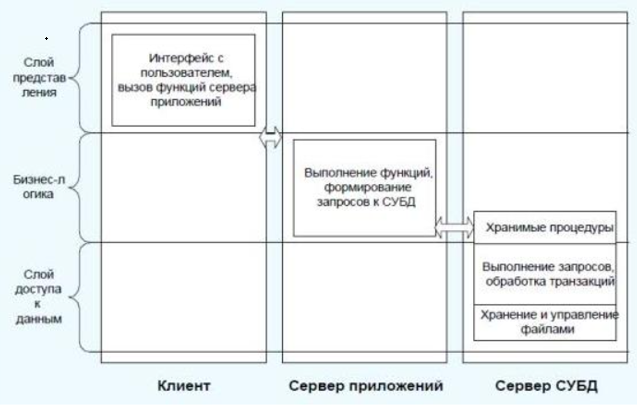
\includegraphics[width=0.8\textwidth]{assets/665}
    \caption{Типичный пример трехзвенной модели}
\end{figure}

Компоненты трехзвенной архитектуры, с точки зрения программного обеспечения
реализуют определенные сервера БД, web-сервера и браузеры. Место любого из этих
компонентов может занять программное обеспечение любого производителя.~\\

Сервер приложений располагается на выделенном сервере приложений, выполняющем функции промежуточного ПО.~\\

Плюсы:
\begin{itemize}
    \item Тонкий клиент.
    \item Между клиентской программой и сервером приложения передается лишь минимально необходимый поток данных - аргументы вызываемых функций и возвращаемые от них значения.
    \item Сервер приложения может быть запущен в одном или нескольких экземплярах на одном или нескольких компьютерах.
    \item Дешевый трафик между сервером приложений и СУБД. Трафик между сервером приложений и СУБД может быть большим, однако это всегда трафик локальной сети, а их пропускная способность достаточно велика и дешева. В крайнем случае, всегда можно запустить СП и СУБД на одной машине, что автоматически сведет сетевой трафик к нулю.
    \item Дешевле наращивать функциональность и обновлять ПО.
\end{itemize}

Минусы:
\begin{itemize}
    \item Более высокая сложность создания приложений.
    \item Сложнее в разворачивании и администрировании.
    \item Высокие требования к производительности серверов приложений и сервера базы данных, а, значит, и высокая стоимость серверного оборудования.
    \item Высокие требования к скорости канала (сети) между сервером базы данных и серверами приложений.
\end{itemize}

\subparagraph{Отличия}~\\

По сравнению с двухзвенной клиент-серверной архитектурой трёхуровневая архитектура
обеспечивает, как правило, большую масштабируемость (за счёт горизонтальной
масштабируемости сервера приложений и мультиплексирования соединений), большую
конфигурируемость (за счёт изолированности уровней друг от друга). Реализация
приложений, доступных из веб-браузера или из тонкого клиента, как правило,
подразумевает развёртывание программного комплекса в трёхуровневой архитектуре. При
этом обычно разработка трёхзвенных программных комплексов сложнее, чем для
двухзвенных, также наличие дополнительного связующего программного обеспечения
может налагать дополнительные издержки в администрировании таких комплексов.~\\

DCE (Distributed Computing Environment)~--- это система программного обеспечения,
предназначенная для разработки программ, использующих распределённые вычисления. \autocite{dce}
Состоит из:
\begin{itemize}
    \item Удалённый вызов процедур (RPC, remote procedure call)~--- DCE имеет собственную систему RPC (DCE/RPC). Как и любой RPC, используется для вызова процедур на удалённом компьютере.
    \item Служба каталогов (Directory Service)~--- центральное хранилище информации о ресурсах в распределённой системе. К ним относятся пользователи, компьютера и службы RPC, а также их атрибуты (свойства).
    \item Служба безопасности (Security Service)~--- служба, отвечающая за защиту данных при передаче по сети (с помощью шифрования, например), контроль доступа к вычислительным ресурсам, и т. д.
    \item Служба синхронизации времени (Time Service)~--- как понятно из названия, используются для синхронизации времени на узлах системы.
    \item Файловая служба (File Service)~--- позволяет пользователям получать доступ к файлам, хранящимся на файловом сервере.
    \item Threads~--- реализует многопоточность, если она не реализована на уровне ОС.
\end{itemize}

Появление сетей ЭВМ позволило наряду с централизованными создавать и распределенные базы данных.
\textbf{Распределенная база данных} состоит из нескольких, возможно, пересекающихся или даже дублирующих друг друга
частей, хранимых в различных ЭВМ вычислительной сети. Однако пользователь распределенной базы данных не обязан
знать, каким образом ее компоненты размещены в узлах сети, и представляет себе эту базу данных как единое
целое. Работа с такой базой данных осуществляется с помощью \textit{системы управления распределенной базой данных} (СУРБД).
Не следует путать распределённую базу данных с репликацией. Репликация~--- это поддержание синхронизированных
копий одних и тех же данных, тогда как распределённая база данных~--- это распределение различных данных по различным серверам.
Распределённая БД тоже может поддерживать репликацию.

Преимущества распределённых БД \autocite{DDBMSIndusEdition}:
\begin{itemize}
    \item Для расширения нужно добавить новый компьютер, а не менять существующую систему.
    \item При отказе одного узла остальные продолжают работать.
    \item Если эффективно распределить данные, можно снизить время ожидания для пользователя и затраты на связь с БД.
\end{itemize}

Недостатки~--- более сложное управление всей системой и накладные расходы на передачу данных.


\subsection{Угрозы безопасности распределенных СУБД}
\paragraph{Угрозы доступности, целостности и конфиденциальности данных. Механизмы противодействия} ~\\

\subsubsection{Угрозы доступности, целостности, конфиденциальности данных}
\textbf{Современный подход к информационной безопасности}

Информационная безопасность - это защита информации и инфраструктуры с помощью различных средств и методов. Комплексный подход включает использование защитных механизмов на всех этапах жизненного цикла системы. При проектировании системы безопасности учитываются передовые тенденции, включая интрасети (Intranet). Защита WEB-сервиса, центрального элемента интрасетей, имеет первостепенное значение.

\bigbreak
\textbf{Угрозы СУБД}

Распределённые системы управления базами данных (СУБД) представляют собой сложную инфраструктуру, которая подвержена различным угрозам безопасности. Эти угрозы могут иметь серьёзные последствия, включая потерю или искажение данных, нарушение конфиденциальности и доступности информации. В этом разделе мы рассмотрим некоторые из ключевых угроз безопасности, связанных с распределёнными СУБД \autocite{DistrDBThreats}.

\textbf{Проблемы синхронизации}

В распределённых СУБД данные хранятся на разных серверах или узлах. Каждый узел обрабатывает свои запросы и обновляет данные. Если эти обновления не синхронизируются должным образом между всеми узлами, это может привести к несоответствию данных. Например, один и тот же запрос, выполненный на разных узлах, может дать разные результаты.

\textbf{Угрозы сетевой безопасности}

Поскольку данные передаются по сети между различными узлами, они подвержены угрозам, таким как перехват данных, атаки "человек посередине" и другие виды сетевых атак. Это может привести к утечке конфиденциальной информации или к нарушению целостности данных.

\textbf{Проблемы доступа и аутентификации}

Управление доступом и аутентификация пользователей в распределённой среде может быть сложной задачей. Если злоумышленник может обойти механизмы аутентификации или контроля доступа, он может получить несанкционированный доступ к данным.

\textbf{Отказ оборудования или сети}

В распределённых СУБД отказ одного из узлов или линии связи между узлами может привести к потере доступа к данным. Это может привести к простоям в работе и потере важной информации.

\textbf{Угрозы целостности данных}

В распределённых СУБД данные часто реплицируются на нескольких серверах для обеспечения отказоустойчивости. Если процесс репликации нарушается, это может повлиять на целостность данных. Например, обновление может быть применено на одном сервере, но не на другом.

\subsubsection{Механизмы противодействия угрозам}
СУБД отличаются от других компонентов ИС специфичными угрозами, и главным их источником является
сама природа баз данных. Известно, что основным средство общения с СУБД выступает язык SQL,
являющийся мощным инструментом манипулирования данными. С его помощью, используя механизм правил, могут
быть созданы сложные, трудно поддающиеся анализу цепочки действий, позволяющие не явным образом передавать
право на выполнение определенных процедур тем, кто не имеет на это полномочий \autocite{DistrDBThreats}.

В качестве примера можно привести несколько угроз, возникающих при использовании языка SQL: получение
информации путем логических выводов, агрегирование данных, покушение на высокую доступность.

Методы борьбы против получения информации путем логических выводов состоят в тщательном проектировании
модели данных, иерархии привилегий и видимых пользователям представлений.

Агрегирование данных состоит в получении новой информации путем комбинирования данных, полученным официальным
путем. Причем информация, содержащаяся в скомбинированных данных, может иметь гриф более высокий, чем первичная информация.

Методом борьбы с агрегированием может быть тщательное проектирование модели данных и максимально допустимое
ограничение доступа пользователей к информации.

Покушение на высокую доступность может быть реализовано, если пользователю-нарушителю доступны все возможности
языка SQL. При этом он легко сможет заблокировать работу других пользователей. Поэтому, в целях борьбы с данным
видом угроз, рекомендуется запрещать непосредственный SQL-доступ к базе данных, используя для этого серверы приложений \autocite{DistrDBThreats}.

В распределённых СУБД необходимо передавать данные между узлами. 
Поэтому, кроме перечисленных угроз, в них также реализуются угрозы, связанные с каналами связи.
Защититься от них можно с помощью шифрования.

В распределённых СУБД пользователи могут обращаться к разным серверам.
Например, первый пользователь обращается к первому серверу БД и просит удалить некоторую строку, которая расположена на втором сервере.
А в это время второй пользователь обращается ко второму серверу и просит прочитать эту строку.
В таком случае может возникнуть ситуация, когда строка уже удалена, но второй пользователь её получил.
Защищаться от этого необходимо с помощью распределённых транзакций.

\bigbreak
\textbf{Средства резервного копирования}

Резервное копирование программ и данных необходимо проводить с целью минимизации потерь в случае отказов
оборудования, либо сбоев в программном обеспечении ИС. Данная задача наиболее сложна именно в интрасетях
с их распределенными ресурсами и неоднородностью, в которых работают компьютеры под управлением различных
операционных систем. Учитывая клиент/серверный характер интрасетей функцию резервного копирования целесообразно
также выделить в виде отдельного сервера (сервера архива).

Распространение клиент/серверного подхода на процедуру резервного копирования информации и данных
имеет ряд преимуществ по сравнению с традиционными методами. Они выражаются в следующем \autocite{DistrDBThreats}:
\begin{itemize}
    \item Администраторы рабочих групп освобождаются от необходимости согласования действий
    и самой процедуры создания локальных резервных копий
    \item Единообразие процедуры создания резервных копий в ИС
    \item Возможность мониторинга процесса резервирования и диагностики возникших проблем
\end{itemize}

Одним из способов обеспечения высокой доступности информации является создание резервных копий с возможностью
ее хранения в двух местах: один экземпляр хранится поблизости от оригинала, а другой в удаленном безопасном месте.


\bigbreak
\textbf{Обеспечение конфиденциальности данных}

В СУБД, как правило, используется произвольное управление доступом, когда владелец объекта передает
права доступа к нему (привилегии) по своему усмотрению. При этом привилегии в СУБД можно подразделить на две
категории: привилегии безопасности и привилегии доступа \autocite{DistrDBThreats}.

Привилегии безопасности всегда выделяются конкретному пользователю и позволяют выполнять административные действия.

Привилегии доступа определяют права доступа субъектов к определенным объектам.

Специфическим механизмом управления доступом в СУБД являются представления. Они позволяют сделать
видимыми для субъектов только те столбцы базовых таблиц, доступ к которым предоставлен субъектам администратором базы.

\bigbreak
\textbf{Поддержание целостности}

Целостность данных не менее важна, чем конфиденциальность, ввиду того, что для баз данных, как и для
ИС в целом, главными врагами являются не внешние нарушители, а ошибки оборудования, программ, администраторов и
пользователей системы \autocite{DistrDBThreats}.

С точки зрения пользователей СУБД, основными средствами поддержания целостности данных являются ограничения и правила.

Ограничения могут относиться как к таблицам, так и к отдельным столбцам. Они накладываются владельцами
таблицы и оказывают влияние на все операции с данными.

Правила позволяют вызывать выполнение заданных действий при определенных изменениях базы данных.
В отличие от ограничений, являющихся лишь средствами контроля простых условий, правила позволяют
создавать сколь угодно сложные соотношения между различными элементами базы данных.

\bigbreak
\textbf{Обеспечение доступности данных}

Доступность данных подразумевает обеспечение информационной системы средствами поддержания высокой
доступности. Поддержание высокой доступности позволяет свести к минимуму возможные сбои аппаратного
обеспечения, в частности носителей информации, а также ошибки обслуживающего персонала и программного
обеспечения. В качестве мер поддержания высокой доступности может быть названа кластеризация сервера баз
данных (выделение нескольких компьютеров, выполняющих общее приложение), а также тиражирование данных
(хранение базы данных в различных местах) \autocite{DistrDBThreats}.




\subsection{Распределенная обработка данных}
\paragraph{Понятие распределенной транзакции}~\\
Если данные хранятся в одной базе данных, то транзакция к ней рассматривается как локальная.
В распределенных базах транзакция, выполнение которой заключается в обновлении данных на нескольких узлах сети,
называется глобальной или \textbf{распределенной транзакцией}.

Внешне выполнение распределенной транзакции выглядит как обработка транзакции к локальной базе данных.
Тем не менее распределенная транзакция включает в себя несколько локальных транзакций, каждая из которых
завершается двумя путями — фиксируется или прерывается. Распределенная транзакция фиксируется только в том случае,
когда зафиксированы все локальные транзакции, ее составляющие.

\paragraph{Модель обработки транзакций} ~\\
В стандарте ANSI/ISO SQL определены модель транзакций и функции операторов COMMIT и ROLLBACK. \autocite{AnsiSqlTrans}
Стандарт определяет, что транзакция начинается с первого SQL-оператора, инициируемого пользователем или содержащегося
в программе. Все последующие SQL-операторы составляют тело транзакции. Транзакция завершается одним из четырех
возможных путей \autoref{ansi_transactions}
\begin{itemize}
    \item оператор COMMIT означает успешное завершение транзакции; его использование делает постоянными изменения,
    внесенные в базу данных в рамках текущей транзакции
    \item оператор ROLLBACK прерывает транзакцию, отменяя изменения, сделанные в базе данных в рамках
    этой транзакции; новая транзакция начинается непосредственно после использования ROLLBACK
    \item успешное завершение программы, в которой была инициирована текущая транзакция,
    означает успешное завершение транзакции (как будто был использован оператор COMMIT)
    \item ошибочное завершение программы прерывает транзакцию (как будто был использован оператор ROLLBACK)
\end{itemize}

\begin{figure}[h!]
    \centering
    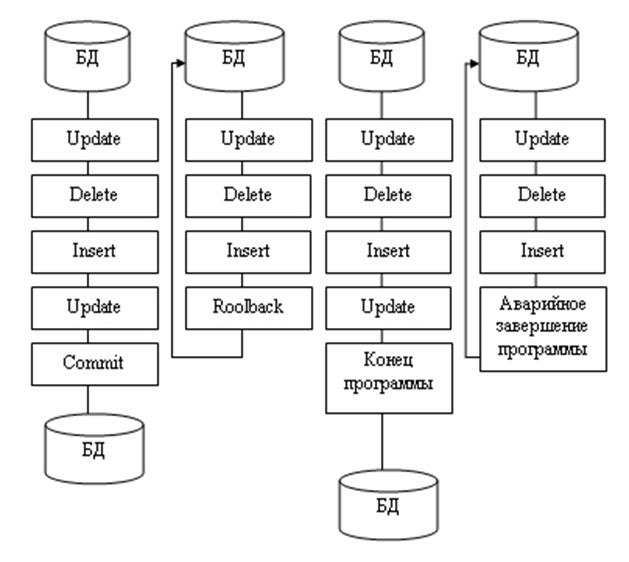
\includegraphics[width=0.8\textwidth]{assets/distributed/transactions.jpg}
    \caption{Модель транзакций ANSI/ISO}
	\label{ansi_transactions}
\end{figure}

Точки сохранения применяются, как правило, в протяженных транзакциях и позволяют разделить транзакцию на несколько
небольших осмысленных фрагментов. Пользователь может зафиксировать работу в любой точке транзакции с тем,
чтобы выполнить ее откат к состоянию, соответствующему этой точке.

Откат и фиксация транзакций становятся возможными благодаря журналу транзакций. Он используется следующим образом.
Известно, что все операции над реляционной базой данных суть операции над строками таблиц. Следовательно,
для обеспечения отката таблиц к предыдущим состояниям достаточно хранить не состояния таблицы, а лишь те
ее строки, которые подверглись изменениям.

При выполнении любого оператора SQL, который вносит изменения в базу данных, СУБД автоматически заносит
очередную запись в журнал транзакций. Запись состоит из двух компонентов: первый - это состояние строки до
внесения изменений, второй - ее же состояние после внесения изменений. Только после записи в журнал транзакций
СУБД действительно вносит изменения в базу данных. Если после данного оператора SQL был выполнен оператор
COMMIT, то в журнале транзакций делается отметка о завершении текущей транзакции. Если же после
оператора SQL следовал оператор ROLLBACK, то СУБД просматривает журнал транзакций и отыскивает записи,
отражающие состояние измененных строк до внесения изменений. Используя их, СУБД восстанавливает те
строки в таблицах базы данных, которые были изменены текущей транзакцией, - таким образом
аннулируются все изменения в базе данных.

\paragraph{Мониторы обработки транзакций}~\\
Мониторы обработки транзакций (Transaction Processing Monitor - TPM), или мониторы
транзакций - программные системы, предназначенные для поддержки выполнения распределённых транзакций.
Они относятся к категории middleware, то есть к ПО, работающему между ОС и приложениями \autocite{TransactionMonitors}.

Это происходит следующим образом: клиент начинает транзакцию и обращается к TPM, который выдаёт ему
идентификатор транзакции и контекст транзакции. Затем клиент с помощью RPC обращается к серверу,
включая контекст в обращение. Сервер извлекает контекст, уведомляет TPM о том, что он (сервер) участвует
в транзакции, и обрабатывает запрос как обычно. Так коиент обращается ко всем необходимым серверам. 
Когда клиент достиг окончания транзакции, он уведомляет об этом TPM, и тот выполняет протокол двухфазного коммита
для всех серверов, участвовавших в транзакции. После завершения протокола TPM уведомляет об этом клиента (Рис. \ref{tpm_process}). \autocite{WebServices}

\begin{figure}[h!]
    \centering
    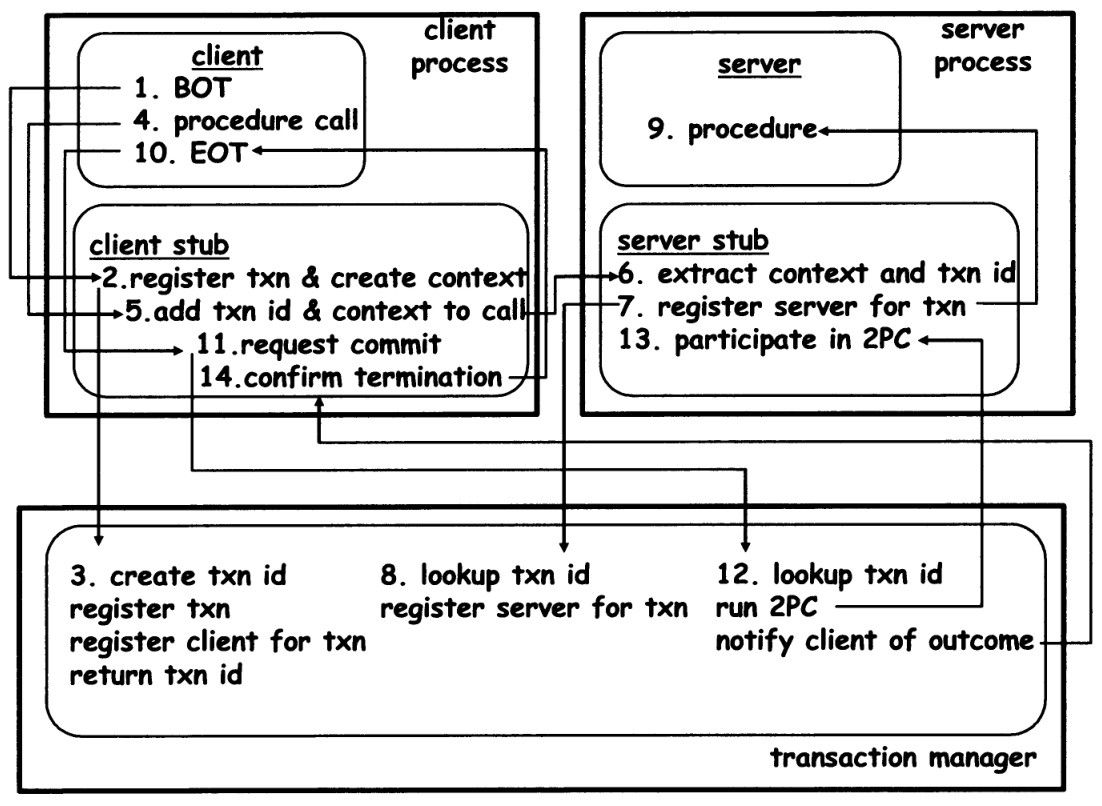
\includegraphics[width=0.8\textwidth]{assets/distributed/TPM_arch.png}
    \caption{Процесс взаимодействия с TPM}
	\label{tpm_process}
\end{figure}

TPM опираются на трехзвенную модель "клиент-сервер" (модель сервера приложений или AS-модель), описанную в Разделе 2.
Естественно, что все преимущества модели отражаются и на программных системах, построенных на ее основе.

На современном рынке мониторов транзакций основными "действующими лицами" являются такие системы,
как ACMS (DEC), CICS (IBM), TOP END (NCR), PATHWAY (Tandem), ENCINA (Transarc), TUXEDO System (USL).
Несмотря на принципиальное сходство, конкретные TPM отличаются рядом характеристик, причем
различия часто вытекают как из специфики операционной системы, в которой реализован и функционирует TPM.

\paragraph{Корпоративная среда обработки транзакций}~\\

TPM на базе UNIX опирается на фундаментальное понятие - корпоративную среду обработки транзакций
(Enterprise Transaction Processing - ETP). Архитектура ETP - это три ряда компьютеров \autocite{TransactionMonitors}:
\begin{itemize}
    \item Ряд 1: Персональные станции (Personal Workstations);
    \item Ряд 2: Компьютеры под управлением ОС UNIX (UNIX Transaction Processing Servers - UPTS);
    \item Ряд 3: Mainframe-системы (Proprietary Transaction Processing Servers - PTPS)
    или компьютеры под управлением UNIX c RISC-архитектурой процессоров;
\end{itemize}

Компьютеры \textbf{ряда 1}, функционирующие под управлением DOS, MS Windows, OS/2, UNIX, используются в качестве рабочих мест
конечных пользователей. Характерная черта ETP - отсутствие ограничений на модели компьютеров,
составляющих этот ряд. Однако, как правило, ряд 1 состоит из компьютеров на базе процессоров Intel
486/Pentium под управлением MS Windows (MS Windows фактически стала стандартом оконного графического интерфейса
для большинства категорий пользователей и стандартом операционной среды для подавляющего числа прикладных программ и систем) \autocite{TransactionMonitors}.

\textbf{Ряд 2} составляют компьютеры среднего класса под управлением ОС UNIX,
на которых функционирует ядро TPM и, как правило, реляционные СУБД (Oracle, Informix, Ingres),
выступающие в качестве менеджера ресурсов. Кроме того, на них же может быть установлен шлюз к TPM в
операционной среде мэйнфрейма (как правило, разработчики TPM на базе UNIX предусматривают в конфигурации своих
систем шлюз к наиболее популярной такой системе - IBM CICS) \autocite{TransactionMonitors}.

\textbf{Ряд 3} представлен мэйнфреймами или RISC-компьютерами под управлением UNIX. О мэйнфреймах мы
говорим в тех ситуациях, когда исторически сложилось так, что в организации они существуют уже долгое время,
берут на себя большую часть всего объема обработки транзакций, концетрируют огромные вычислительные
ресурсы и содержат большие массивы данных (то есть речь идет об унаследованных системах). Если этого
"тяжелого наследия" нет, то можно смело использовать в качестве компьютеров ряда 3 RISC-серверы,
сегодня приближающиеся по производительности к мэйнфреймам \autocite{TransactionMonitors}.

Таким образом, среда обработки транзакций формируется из набора разнородных компьютеров (и соответствующих ОС),
ранжируемых от персональных компьютеров до мэйнфрейм-систем. TPM на базе UNIX представляет собой своего
рода "клей", который связывает вместе компьютеры трех рядов в открытую унифицированную среду обработки транзакций.

Ключом к интеграции систем, функционирующих на компьютерах различных рядов, является специализированный
интерфейс прикладного программирования ATMI (Application Transaction Manager Interface), обеспечивающий \autocite{TransactionMonitors}:
\begin{itemize}
    \item для ряда 1 - формирование и передачу запросов от клиентов к серверам, выполняющимся на компьютерах ряда 2
    \item для ряда 2 - обработку запросов, поступающих от компьютера ряда 1 (в том числе и с
    обращением к менеджеру ресурсов), и, по необходимости, формирование и направление
    запросов к серверам, выполняющимся на компьютерах ряда 3
    \item для ряда 3 - обработку запросов, поступающих от серверов ряда 2
\end{itemize}

Стоит отметить, что подобное представление о корпоративной среде обработки транзакций не является абстракцией.
Сегодня многие организации приходят именно к такой, "трехуровневой"  архитектуре информационных
систем (с той оговоркой, что наличие ряда 3 вызвано историческими причинами - мэйнфреймы использовались
первоначально и сразу от них отказаться невозможно).

\subsection{Протоколы фиксации}
\paragraph{Протоколы фиксации}~\\
Протоколы фиксации используются для обеспечения атомарности транзакций между сайтами.
Транзакция, которая выполняется на нескольких сайтах, должна быть либо зафиксирована на всех сайтах, либо прервана на всех сайтах.
Недопустимо, чтобы транзакция была зафиксирована на одном сайте и прервана на другом.
В локальной системе базы данных для принятия транзакции диспетчер транзакций должен только передать решение
о фиксации диспетчеру восстановления. Однако в распределенной системе диспетчер транзакций должен передать
решение о фиксации всем серверам в различных сайтах, где выполняется транзакция, и обеспечить
единообразное выполнение решения. Когда обработка завершается на каждом сайте, она достигает состояния
частично подтвержденной транзакции и ожидает, пока все другие транзакции достигнут их частично подтвержденных состояний.
Когда он получает сообщение о том, что все сайты готовы к фиксации, он начинает фиксировать.
В распределенной системе либо все сайты фиксируют, либо ни один из них не делает \autocite{FixProtocols}.

Различные протоколы распределенной фиксации \autocite{FixProtocols}:
\begin{itemize}
    \item Однофазный коммит
    \item Двухфазный коммит
    \item Трехфазный коммит
\end{itemize}
Широко используется протокол двухфазной фиксации (2PC).
\bigbreak
\textbf{Распределенная однофазная фиксация}

Распределенная однофазная фиксация – это самый простой протокол фиксации. Давайте рассмотрим, что есть
контролирующий сайт и несколько подчиненных сайтов, где выполняется транзакция. Шаги в распределенном коммите \autocite{FixProtocols}:
\begin{itemize}
    \item После того, как каждое ведомое устройство локально завершило свою транзакцию, оно
    отправляет сообщение «ГОТОВО» на контролирующий сайт
    \item Подчиненные ожидают сообщения «Подтвердить» или «Прервать» с контролирующего сайта.
    Это время ожидания называется окном уязвимости
    \item Когда контролирующий сайт получает сообщение «СДЕЛАНО» от каждого ведомого, он принимает решение
    о фиксации или отмене. Это называется точкой фиксации. Затем он отправляет это сообщение всем рабам
    \item При получении этого сообщения ведомое устройство либо фиксирует, либо прерывает работу,
    а затем отправляет подтверждающее сообщение на контролирующий сайт
\end{itemize}

После того, как каждое ведомое устройство локально завершило свою транзакцию, оно отправляет сообщение
«ГОТОВО» на контролирующий сайт.

Подчиненные ожидают сообщения «Подтвердить» или «Прервать» с контролирующего сайта. Это время ожидания
называется окном уязвимости.

Когда контролирующий сайт получает сообщение «СДЕЛАНО» от каждого ведомого, он принимает решение о
фиксации или отмене. Это называется точкой фиксации. Затем он отправляет это сообщение всем рабам.

При получении этого сообщения ведомое устройство либо фиксирует, либо прерывает работу,
а затем отправляет подтверждающее сообщение на контролирующий сайт.

\bigbreak
\textbf{Распределенная двухфазная фиксация}
Распределенная двухфазная фиксация снижает уязвимость однофазных протоколов фиксации. Шаги, выполняемые на двух этапах \autocite{FixProtocols}:
\bigbreak
\textbf{Этап 1}
\begin{itemize}
    \item После того, как каждое ведомое устройство локально завершило свою транзакцию,
    оно отправляет сообщение «ГОТОВО» на контролирующий сайт. Когда контролирующий сайт получил сообщение «ГОТОВО»
    от всех подчиненных, он отправляет сообщение «Подготовить» подчиненным
    \item Рабы голосуют за то, хотят ли они по-прежнему совершать или нет. Если ведомый
    хочет зафиксировать, он отправляет сообщение «Готово»
    \item Раб, который не хочет коммитить, отправляет сообщение «Не готов». Это может произойти,
    если ведомое устройство имеет конфликтующие параллельные транзакции или истекло время ожидания
\end{itemize}

После того, как каждое ведомое устройство локально завершило свою транзакцию, оно отправляет
сообщение «ГОТОВО» на контролирующий сайт. Когда контролирующий сайт получил сообщение «ГОТОВО» от всех подчиненных,
он отправляет сообщение «Подготовить» подчиненным.

Рабы голосуют за то, хотят ли они по-прежнему совершать или нет. Если ведомый хочет зафиксировать,
он отправляет сообщение «Готово».

Раб, который не хочет коммитить, отправляет сообщение «Не готов». Это может произойти, если ведомое
устройство имеет конфликтующие параллельные транзакции или истекло время ожидания.

\textbf{Этап 2}

\begin{itemize}
    \item После того, как контролирующий сайт получил сообщение «Готово» от всех ведомых \autocite{FixProtocols} –
    \begin{itemize}
        \item Контролирующий сайт отправляет сообщение «Global Commit» подчиненным
        \item Подчиненные устройства применяют транзакцию и отправляют сообщение «Подтвердить ACK» на контролирующий сайт
        \item Когда контролирующий сайт получает сообщение «Подтвердить ACK» от всех ведомых
        устройств, он считает транзакцию подтвержденной
    \end{itemize}
    \item После того, как контролирующий сайт получил первое сообщение «Не готов» от любого ведомого –
    \begin{itemize}
        \item Контролирующий сайт отправляет сообщение «Global Abort» подчиненным
        \item Слэйвы отменяют транзакцию и отправляют сообщение «Abort ACK» на контролирующий сайт
        \item Когда контролирующий сайт получает сообщение «Abort ACK» от всех ведомых
        устройств, он считает транзакцию отмененной
    \end{itemize}

\end{itemize}
\textbf{Обработка отказов}

Введём следующие обозначения: T -- транзакция, инициированная сайтом $S_i$, координатором которого выступает $C_i$.

\begin{itemize}
\item Отказ сайта

Когда сайт восстанавливается, он просматривает свой журнал, чтобы определить судьбу транзакций, активных во время сбоя\autocite{Fixations}:
\begin{itemize}
\item Журнал содержит запись <commit T>: сайт выполняет переотправку (T)
\item Журнал содержит запись <abort T>: сайт выполняет отмену (T)
\item Журнал содержит запись <ready T>: сайт должен обратиться к $C_i$, чтобы определить судьбу T.
\begin{itemize}
\item Если T зафиксировано, повторить (T)
\item Если Т прервано, отмена (Т).
\end{itemize}
\item Журнал не содержит никаких управляющих записей относительно ответов T что $S_k$ потерпел неудачу, прежде чем ответил на сообщение prepare T от $C_i$
\begin{itemize}
\item поскольку отказ $S_k$ исключает отправку такого ответа $C_1$ должен прервать T
\item $S_k$ должен выполнить отмену (T)
\end{itemize}
\end{itemize}  

\item Отказ координатора

Если координатор вышел из строя во время выполнения протокола фиксации для T то участвующие сайты должны принять решение о дальнейшей судьбе T\autocite{Fixations}:
\begin{itemize}
\item Если активный сайт содержит запись <commit T> в своем журнале, то T должен быть зафиксирован.
\item Если активный сайт содержит в своем журнале запись <abort T>, то T должен быть прерван.
\item Если какой-либо активный участвующий сайт не содержит записи <ready T> в своем журнале, тогда отказавший координатор $C_i$ не может принять решение о фиксации T. Поэтому можно прервать T.
\item Если ни один из вышеперечисленных случаев не подходит, то все активные сайты должны иметь запись <ready T> в своих журналах, но никаких дополнительных управляющих записей (таких как <abort T> из <commit T>). В этом случае активные сайты должны ждать, пока $C_i$ восстановится, чтобы найти решение.
\item Проблема блокировки: активным сайтам, возможно, придется ждать, пока вышедший из строя координатора будет восстановлен.
\end{itemize}
\item Разделение сети

Если координатор и все его участники остаются в одном разделе, отказ не влияет на протокол фиксации.\autocite{Fixations}
Если координатор и его участники принадлежат к нескольким разделам:
\begin{itemize}
\item Сайты, которые не находятся в разделе, содержащем координатора считают, что координатор вышел из строя, и выполняют протокол, соответствующий случаю отказа координатора.

\end{itemize}
Координатор и сайты, находящиеся в том же разделе, что и координатор считают, что сайты в другом разделе отказали, и следуют обычному протоколу фиксации.


\end{itemize}

\bigbreak
\textbf{Контролирование управления и параллелизма}

В случае обработки in-doubt (т.е. таких, о которых в логах есть запись <ready T>, но нет ни <commit T>, ни <abort T>) транзакций восстанавливающий сайт должен определить её commit-abort статус контактируя с другими сайтами, что может замедлить и, возможно, заблокировать процесс востановления\autocite{Fixations}.

Опишем основные принципы работы алгоритмов восстановления:
\begin{itemize}
    \item Алгоритмы могут записывать информацию о фиксациях в лог.
    \item Вместо <ready T> вносится запись <ready T, L>, где L -- список фиксаций, удерживаемых транзакцие T при записи лога, причём фиксации чтения могут быть опущены.
    \item Для каждой in-doubt транзакции T все фиксации, записанные в <ready T, L> запрашиваются снова.
    \item После повторного получения фиксации обработка транзакции может быть продолжена, при этом фиксация/откат in-doubt транзакции выполняется параллельно с исполнением новых транзакций.
\end{itemize}

\bigbreak
\textbf{Распределенная трехфазная фиксация}
Шаги в распределенной трехфазной фиксации следующие \autocite{FixProtocols}:
\begin{itemize}
    \item Этап 1: Шаги такие же, как при распределенной двухфазной фиксации
    \item Этап 2: Подготовьтесь к фиксации
    \begin{itemize}
        \item Контролирующий сайт выдает широковещательное сообщение «Ввод подготовленного состояния»
        \item Ведомые сайты голосуют «ОК» в ответ
    \end{itemize}
    \item Фиксация / Отмена
\end{itemize}

Этапы аналогичны двухфазной фиксации, за исключением того, что сообщение «Подтвердить ACK» / «Прервать ACK» не требуется

\paragraph{Защищенные протоколы фиксации}
\paragraph{Обработка распределенных транзакций в базах данных с многоуровневой секретностью (MLS)}~\\
Известно, что в MLS/DBMS не ко всем данным, содержащимся в  базе
данных, доступ осуществляется одинаково. Однако современные СУБД, как
правило,  не имеют адекватных средств диагностики и механизма определения
того, что пользователь имеет возможность доступа только  к  тем
данным,  которые являются релевантными. Таким образом, MLS/DBMS отличается
от соответствующих DBMS,  по крайней  мере,  следующими  двумя
особенностями \autocite{SecureFix}:
\begin{itemize}
    \item каждый элемент данных в базе данных связан с уровнем доступа
    \item доступ пользователя к данным должен контролироваться релевантностью для данного пользователя
\end{itemize}
Разработка сервиса MLS/DBMS в современных компьютерных  системах
представляет  много  проблем. До настоящего времени внедрение многоуровневого
разграничения доступа в операционную  систему  представляет
собой  значительные трудности. Решение этой проблемы в виде аббревиатуры
обозначается ТСВ. Хотя в разрешении вопросов ТСВ  для  удаленных
пользователей  в  MLS/DBMS вводятся компромиссы, остается много проблем,
которые требуется разрешать. Наиболее очевидная проблема состоит
в том, что вопросы классификации в СУБД значительно  сложнее,  чем  в
файловых  системах  и могут быть сложнее реализованы. Другая проблема
состоит в том, что для классификации данных,  содержащих  контекстные
представления,  временные параметры, их композицию, необходимы унифицированные базы данных \autocite{SecureFix}.

\subsection{Тиражирование данных}
\textbf{Тиражирование данных} - это асинхронный перенос изменений объектов исходной базы данных (source database)
в базы данных, принадлежащие к различным узлам распределенной системы. Тиражирование данных может происходит
двумя различными способами: \textbf{шардингом} (или, иначе говоря, шардированием, фрагментацией) и \textbf{репликацией}.

\subsubsection{Шардинг (sharding)}

\textbf{Шардинг} — это метод проектирования базы данных, при котором данные разделяются на группы и хранятся на разных серверах. Это улучшает производительность, поскольку данные хранятся там, где они чаще всего используются, что уменьшает сетевой трафик.

Существуют два основных вида шардирования: \textbf{горизонтальное} и \textbf{вертикальное}. Они соответствуют операциям сокращения и проекции в реляционных базах данных. Важно, чтобы все фрагменты были независимыми, то есть ни один из фрагментов не может быть представлен как производный от других фрагментов.

Одной из ключевых особенностей шардинга является поддержка независимости от шардирования. Это означает, что пользователи могут работать так, как если бы данные в действительности были вовсе не шардированы. Это упрощает разработку пользовательских программ и выполнение терминальных операций.

Если обеспечивается независимость от шардирования, пользователи получают данные в виде представления, в котором шарды логически скомбинированы с помощью операций соединения и объединения. Задачей системного оптимизатора является определение шардов, к которым требуется доступ для выполнения запросов пользователя.
\autocite{IntroBD2014}

\paragraph{Алгоритмы шардинга} ~\\
Ранее уже упоминалось о двух основных вида шардинга: \textit{горизонтальный} и \textit{вертикальный}. Стоит их разобрать по подробнее и
рассказать и про другие виды шардирования, такие как шадинг на основе каталогов и шардинг на основе ключей.

\paragraph{Горизонтальное шардирование} ~\\
В этом методе мы разбиваем данные на основе диапазонов заданного значения, присущего каждой сущности. Допустим, у вас
есть база данных имен ваших онлайн-клиентов и информации об электронной почте. Вы можете разделить эту информацию на
два осколка. В одном осколке вы можете хранить информацию о клиентах, чье имя начинается с A-P, а в другом - информацию
об остальных клиентах.

\begin{figure}[H]
    \centering
    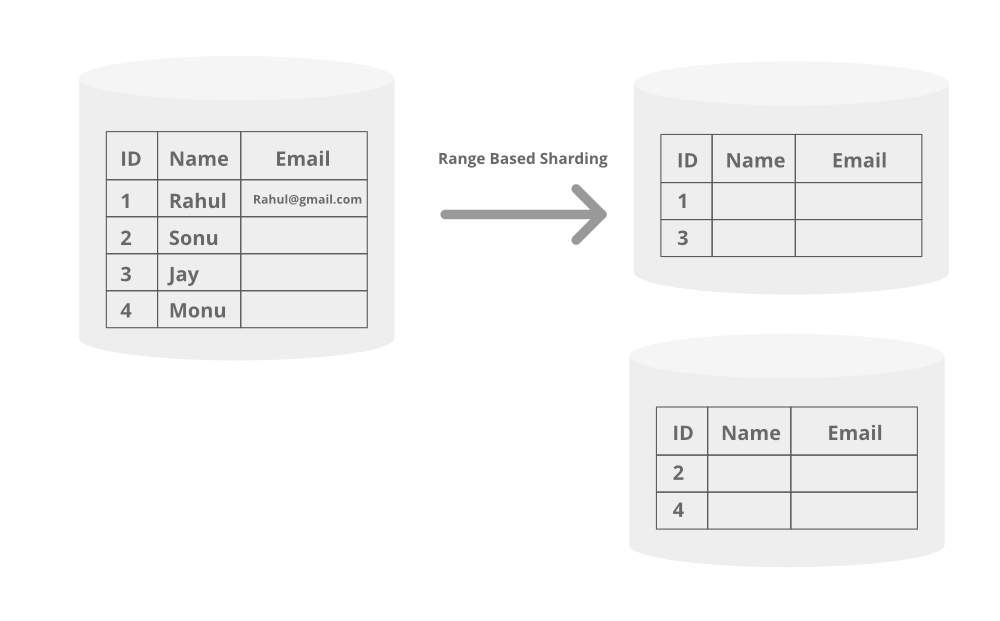
\includegraphics[width=100mm]{assets/distributed/Horizontal-Sharding}
    \caption{Горизонтальное шардирование}
    \label{fig:Horizontal-Sharding}
\end{figure}

\textbf{Горизонтальное шардирование} - самый простой метод сегментирования для реализации. Каждый осколок содержит
другой набор данных, но все они имеют ту же схему, что и исходная база данных. В этом методе вам просто нужно
определить, в какой диапазон попадают ваши данные, а затем вы можете сохранить запись в соответствующий шард. Этот
метод лучше всего подходит для хранения нестатических данных (например, хранение контактной информации студентов
колледжа).

Недостатком этого метода является то, что данные могут быть неравномерно распределены по шардам. В приведенном выше
примере у вас может быть много клиентов, имена которых попадают в категорию A-P. В таких случаях первый осколок должен
будет взять на себя больше нагрузки, чем второй, и это может стать узким местом системы. \autocite{DatabaseSharding}

\paragraph{Вертикальное шардирование} ~\\
В этом методе мы разделяем весь столбец из таблицы и помещаем эти столбцы в новые отдельные таблицы. Данные полностью
независимы от одного раздела к другому. Кроме того, каждый раздел содержит как отдельные строки, так и столбцы. Возьмем,
к примеру, функции Twitter. Мы можем разделить различные функции объекта на разные сегменты на разных машинах. В
Твиттере у пользователя может быть профиль, количество подписчиков и некоторые твиты, опубликованные им самим. Мы можем
разместить профили пользователей на одном осколке, подписчиков - на втором, а твиты - на третьем.

\begin{figure}[H]
    \centering
    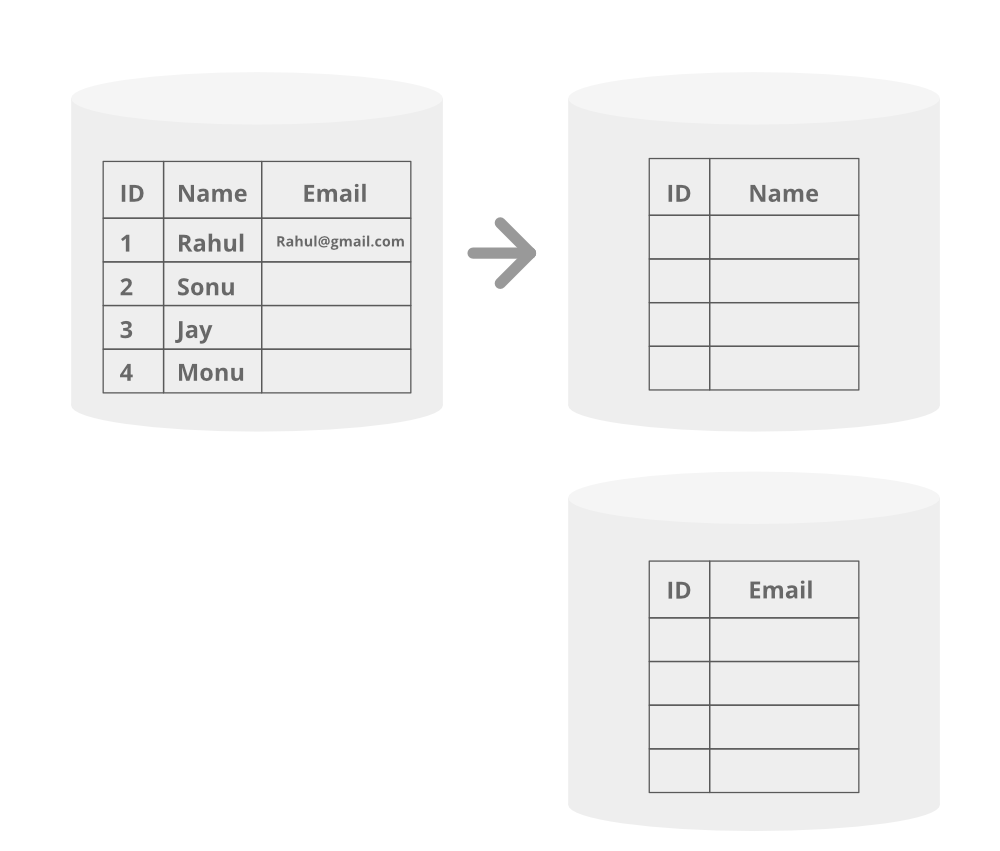
\includegraphics[width=100mm]{assets/distributed/Vertical-Sharding}
    \caption{Вертикальное шардирование}
    \label{fig:Vertical-Sharding}
\end{figure}

В этом методе вы можете отделить и обработать критическую часть (например, профили пользователей) от некритической части
ваших данных (например, сообщения в блоге) по отдельности и построить вокруг нее различные модели репликации и
согласованности. Это одно из главных преимуществ этого метода.

Основным недостатком этой схемы является то, что для ответа на некоторые запросы вам, возможно, придется комбинировать
данные из разных шардов, что неоправданно увеличивает сложность разработки и эксплуатации системы. Кроме того, если
ваше приложение будет расти позже, и вы добавите в него еще несколько функций, вам придется дополнительно сегментировать
базу данных с конкретными функциями на нескольких серверах. \autocite{DatabaseSharding}

\paragraph{Шардинг на основе каталогов} ~\\
В этом методе мы создаем и поддерживаем службу поиска или таблицу поиска для исходной базы данных. В основном мы
используем ключ осколка для таблицы поиска и делаем сопоставление для каждого объекта, существующего в базе данных.
Таким образом, мы отслеживаем, какие осколки базы данных содержат какие данные.

Таблица поиска содержит статический набор информации о том, где можно найти конкретные данные. На приведенном выше
изображении вы можете видеть, что мы использовали зону доставки в качестве ключа осколка. Во-первых, клиентское
приложение запрашивает службу поиска, чтобы узнать осколок (раздел базы данных), на котором размещены данные. Когда
служба поиска возвращает осколок, она запрашивает/обновляет этот осколок.

\begin{figure}[H]
    \centering
    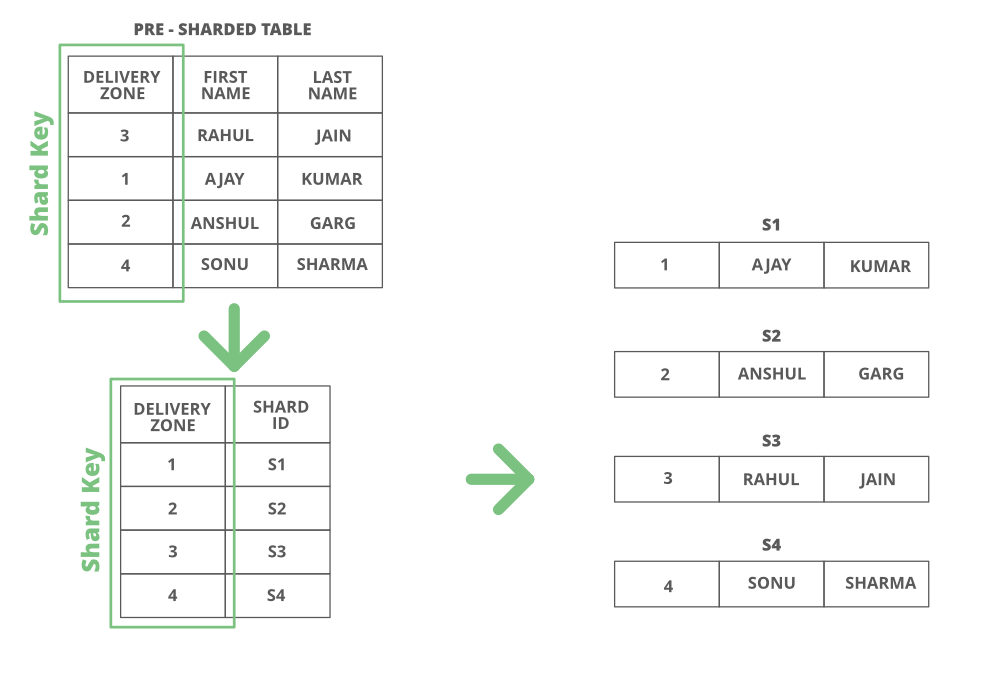
\includegraphics[width=100mm]{assets/distributed/Directory-Based-Sharding}
    \caption{Шардинг на основе каталогов}
    \label{fig:Directory-Based-Sharding}
\end{figure}

Сегментация на основе каталогов гораздо более гибкая, чем сегментация на основе диапазонов и ключей. В сегменте на
основе диапазонов вы обязаны указать диапазоны значений. В key-based вы обязаны использовать фиксированную хэш-функцию,
которую трудно изменить позже. При таком подходе вы можете использовать любой алгоритм, который хотите назначить для
записей данных в сегменты. Кроме того, при таком подходе легко динамически добавлять шарды.

Основным недостатком этого подхода является единственная точка отказа таблицы поиска. Если он будет поврежден или не
удался, это повлияет на запись новых данных или доступ к существующим данным из таблицы. \autocite{DatabaseSharding}

\paragraph{Шардинг на основе ключей} ~\\
Этот метод также известен как сегментация на основе хэша. Здесь мы берем значение объекта, такого как идентификатор
клиента, адрес электронной почты клиента, IP-адрес клиента, почтовый индекс и т. д., и мы используем это значение в
качестве входных данных хэш-функции. Этот процесс генерирует хэш-значение, которое используется для определения того,
какой шард нам нужно использовать для хранения данных. Мы должны иметь в виду, что значения, введенные в хэш-функцию,
должны поступать из одного и того же столбца (ключ осколка), чтобы данные размещались в правильном порядке и
согласованно. В принципе, ключи осколков действуют как первичный ключ или уникальный идентификатор для отдельных строк.

\begin{figure}[H]
    \centering
    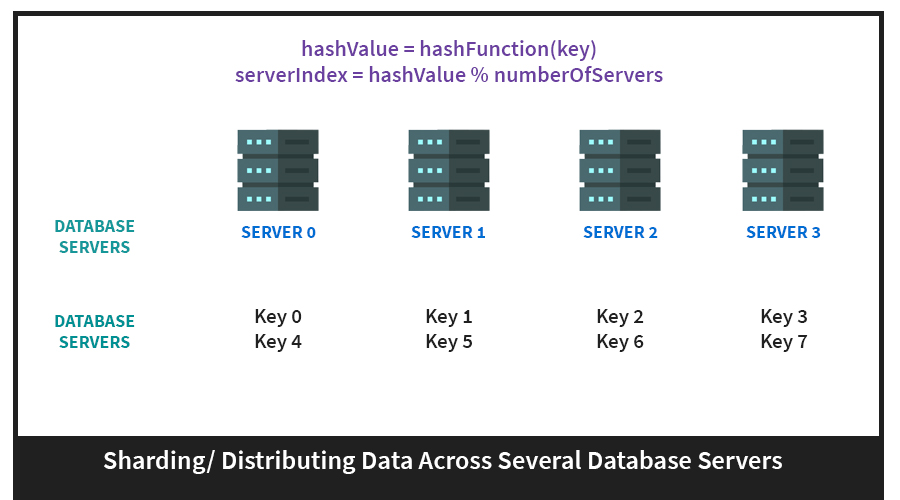
\includegraphics[width=100mm]{assets/distributed/Keybased-Sharding}
    \caption{Шардинг на основе ключей}
    \label{fig:Keybased-Sharding}
\end{figure}

Рассмотрим пример, что у вас есть 3 сервера баз данных, и каждый запрос имеет идентификатор приложения, который
увеличивается на 1 каждый раз, когда регистрируется новое приложение. Чтобы определить, на каком сервере должны быть
размещены данные, мы выполняем операцию по модулю для этих приложений id с номером 3. Затем остаток используется для
идентификации сервера для хранения наших данных.

Недостатком этого метода является эластичная балансировка нагрузки, что означает, если вы попытаетесь динамически
добавлять или удалять серверы баз данных, это будет сложный и дорогостоящий процесс. Например, в приведенном выше
примере, если вы добавите еще 5 серверов, вам нужно добавить больше соответствующих хэш-значений для дополнительных
записей. Кроме того, большинство существующих ключей необходимо переназначить на их новое, правильное хэш-значение,
а затем перенести на новый сервер. Хэш-функция должна быть изменена с модуля 3 на модуль 8. В то время как миграция
данных действует, как новые, так и старые хэш-функции не будут действительны. Во время миграции ваше приложение не
сможет обслуживать большое количество запросов, и вы будете испытывать простои для своего приложения до завершения
миграции. \autocite{DatabaseSharding}

\paragraph{Географический шардинг} ~\\
Шардирование по географическому признаку позволяет хранить определенные данные вблизи своих потребителей и
удовлетворять нормативным требованиям, когда данные должны находиться в определенной юрисдикции. Однако данный способ
шардирования не является самодостаточным: шарды могут быть загружены не равномерно, и отличие может быть на порядки.
На пример, экземпляр базы данных, хранящий данные пользователей Москвы и Московской области, будет намного превышать
другой экземпляр базы данных, который хранит информацию о пользователях из Владимира. Таким образом, недостатком
данного метода является необходимость дополнительного использования других методов шардирования.

\subsubsection{Репликация} ~\\
\textbf{Репликация} — это процесс изменения одного набора данных, называемого репликой, в ответ на изменения другого
набора данных, называемого основным. Репликация желательна по крайней мере по двум причинам. Во-первых, она способна
обеспечить более высокую производительность, поскольку приложения смогут обрабатывать локальные копии вместо того,
чтобы устанавливать связь с удаленными узлами. Во-вторых, наличие репликации может также обеспечивать более высокую
степень доступности, поскольку любой реплицируемый объект остается доступным для обработки (по крайней мере, для выборки
данных), пока хотя бы одна реплика в системе остается доступной. Главным недостатком репликации, безусловно, является
то, что если реплицируемый объект обновляется, то и все его копии должны быть обновлены (проблема распространения
обновлений).

Очевидно, что репликация, как и шардирование, теоретически должна быть "прозрачной для пользователя". Другими словами,
система, которая поддерживает репликацию данных, должна также поддерживать независимость от репликации (иногда говорят
"прозрачность репликации"). Для пользователей должна быть создана такая среда, чтобы они, по крайней мере, с логической
точки зрения могли считать, что в действительности данные не дублируются. Независимость от репликации (как и
независимость от шардирования) является весьма желательной, поскольку она упрощает создание пользовательских программ и
выполнение терминальных операций. В частности, независимость от репликации позволяет создавать и уничтожать дубликаты в
любой момент в соответствии с изменяющимися требованиями, не затрагивая при этом никакие из пользовательских программ
или терминальных операций.

Из требования независимости от репликации следует, что к обязанностям системного оптимизатора также относится
определение, какой именно из физических дубликатов будет применен для доступа к данным при выполнении каждого
введенного пользователем запроса. \autocite{IntroBD2014}

Можно выделить три \textbf{подхода к репликации}:
\begin{itemize}
    \item Блочная репликация на уровне системы хранения данных;
    \item Физическая репликация на уровне СУБД;
    \item Логическая репликация на уровне СУБД.
\end{itemize}

\paragraph{Блочная репликация} ~\\
При блочной репликации каждая операция записи выполняется не только на основном диске, но и на резервном. Таким образом
тому на одном массиве соответствует зеркальный том на другом массиве, с точностью до байта повторяющий основной том.

К достоинствам такой репликации можно отнести простоту настройки и надёжность. Записывать данные на удалённый диск может
либо дисковый массив, либо нечто (устройство или программное обеспечение), стоящее между хостом и диском. Если дисковый
массив не способен реплицировать данные, между хостом и массивом может быть установлен агент, осуществляющей запись на
два массива сразу. Агент может быть как отдельным устройством, так и программным компонентом. В отличие от дискового
массива, который может работать только с таким же массивом или, как минимум, с массивом того же производителя, агент
может работать с совершенно разными дисковыми устройствами.

Главное назначение блочной репликации – обеспечение отказоустойчивости. Если база данных потеряна, то можно
перезапустить её с использованием зеркального тома. Блочная репликация хороша своей универсальностью, но за
универсальность приходится платить.

Во-первых, никакой сервер не может работать с зеркальным томом, поскольку его операционная система не может управлять
записью на него; с точки зрения наблюдателя данные на зеркальном томе появляются сами собой. В случае аварии (отказ
основного сервера или всего ЦОДа, где находится основной сервер) следует остановить репликацию, размонтировать основной
том и смонтировать зеркальный том. Как только появится возможность, следует перезапустить репликацию в обратном
направлении.

Во-вторых, сама СУБД на резервном сервере может быть запущена только после монтирования диска. В некоторых операционных
системах, например, в Solaris, память под кеш при выделении размечается, и время разметки пропорционально объёму
выделяемой памяти, то есть старт экземпляра будет отнюдь не мгновенным. Плюс ко всему кеш после рестарта будет пуст.

В-третьих, после запуска на резервном сервере СУБД обнаружит, что данные на диске неконсистентны, и нужно потратить
значительное время на восстановление с применением журналов повторного выполнения: сначала повторить те транзакции,
результаты которых сохранились в журнале, но не успели сохраниться в файлы данных, а потом откатить транзакции, которые
к моменту сбоя не успели завершиться. \autocite{Replication}

\paragraph{Физическая репликация (master-slave)} ~\\
Журналы (redo log или write-ahead log) содержат все изменения, которые вносятся в файлы базы данных. Идея физической
репликации состоит в том, что изменения из журналов повторно выполняются в другой базе (реплике), и таким образом данные
в реплике повторяют данные в основной базе байт-в-байт \autocite{PhysLogPeplic}.

Журналы СУБД не предназначены для использования вне этой платформы, их формат не документируется и может меняться без
предупреждения. Отсюда совершенно естественное требование, что физическая репликация возможна только между экземплярами
одной и той же версии одной той же СУБД. Отсюда же возможные ограничения на операционную систему и архитектуру
процессора, которые тоже могут влиять на формат журнала.

Естественно, никаких ограничений на модели СХД физическая репликация не накладывает. Более того, файлы в базе-реплике
могут располагаться совсем по-другому, чем на базе-источнике – надо лишь описать соответствие между томами, на которых
лежат эти файлы.

Запись данных в реплику невозможна, поскольку изменения в неё приходят побайтно, и реплика не может обеспечить
конкурентное исполнение своих запросов. В случае повреждения файла в основной базе можно просто скопировать
соответствующий файл с реплики. Однако стоит учесть, что файл на реплике может быть не идентичен файлу в основной базе:
когда файл расширяется, новые блоки в целях ускорения ничем не заполняются, и их содержимое случайно. База может
использовать не всё пространство блока (например, в блоке может оставаться свободное место), но содержимое
использованного пространства совпадает с точностью до байта \autocite{PhysLogPeplic}.

Физическая репликация может быть как синхронной, так и асинхронной. При асинхронной репликации всегда есть некий набор
транзакций, которые завершены на основной базе, но ещё не дошли до резервной, и в случае перехода на резервную базу при
сбое основной эти транзакции будут потеряны. При синхронной репликации завершение операции commit означает, что все
журнальные записи, относящиеся к данной транзакции, переданы на реплику. Важно понимать, что получение репликой журнала
не означает применения изменений к данным. При потере основной базы транзакции не будут потеряны, но если приложение
пишет данные в основную базу и считывает их из реплики, то у него есть шанс получить старую версию этих данных \autocite{PhysLogPeplic}.

Физическая репликация базы данных имеет множество преимуществ перед репликацией средствами СХД \autocite{PhysLogPeplic}:
\begin{itemize}
    \item объём передаваемых данных меньше за счёт того, что передаются только журналы, но не файлы с данными; эксперименты показывают уменьшение трафика в 5-7 раз;
    \item переключение на резервную базу происходит значительно быстрее: экземпляр-реплика уже поднят, поэтому при переключении ему нужно лишь откатить активные транзакции; более того, к моменту сбоя кеш реплики уже прогрет;
    \item на реплике можно выполнять запросы, сняв тем самым часть нагрузки с основной базы. В частности, реплику можно использовать для создания резервных копий.
\end{itemize}

\paragraph{Логическая репликация (active-active)} ~\\
Все изменения в базе данных происходят в результате вызовов её API – например, в результате выполнения SQL-запросов.
Очень заманчивой кажется идея выполнять одну и ту же последовательность запросов на двух разных базах. Для репликации
необходимо придерживаться двух правил \autocite{PhysLogPeplic}:
\begin{itemize}
    \item нельзя начинать транзакцию, пока не завершены все транзакции, которые должны закончиться раньше; Так на рисунке ниже нельзя запускать транзакцию D, пока не завершены транзакции A и B;
    \item нельзя завершать транзакцию, пока не начаты все транзакции, которые должны закончиться до завершения текущей транзакции; Так на рисунке ниже даже если транзакция B выполнилась мгновенно, завершить её можно только после того, как начнётся транзакция C.
\end{itemize}

\begin{figure}[H]
    \centering
    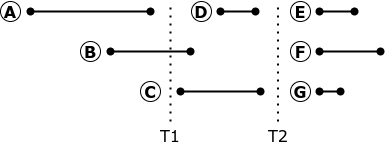
\includegraphics[width=100mm]{assets/distributed/ReplicationExample}
    \caption{Пример репликации}
    \label{fig:ReplicationExample}
\end{figure}

\textbf{Репликация команд (statement-based replication)} реализована, например, в MySQL. К сожалению, эта простая схема не
приводит к появлению идентичных наборов данных – тому есть две причины \autocite{PhysLogPeplic}.
\begin{itemize}
    \item не все API детерминированы. Например, если в SQL-запросе встречается функция now() или sysdate(), возвращающая текущее время, то на разных серверах она вернёт разный результат – из-за того, что запросы выполняются не одновременно. Кроме того, к различиям могут привести разные состояния триггеров и хранимых функций, разные национальные настройки, влияющие на порядок сортировки, и многое другое.
    \item репликацию, основанную на параллельном исполнении команд, невозможно корректно приостановить и перезапустить. На рисунке выше если репликация остановлена в момент T1 транзакция B должна быть прервана и откачена. При перезапуске репликации исполнение транзакции B может привести реплику к состоянию, отличному от состояния базы-источника: на источнике транзакция B началась до того, как закончилась транзакция A, а значит, она не видела изменений, сделанных транзакцией A. Репликация запросов может быть остановлена и перезапущена только в момент T2, когда в базе нет ни одной активной транзакции. Разумеется, на сколько-нибудь нагруженной промышленной базе таких моментов не бывает.
\end{itemize}

Обычно для логической репликации используют детерминированные запросы. Детерминированность запроса обеспечивается двумя
свойствами:
\begin{itemize}
    \item запрос обновляет (или вставляет, или удаляет) единственную запись, идентифицируя её по первичному (или уникальному) ключу;
    \item все параметры запроса явно заданы в самом запросе.
\end{itemize}

В отличие от \textbf{репликации команд (statement-based replication)} такой подход называется \textbf{репликацией
записей (row-based replication)} \autocite{PhysLogPeplic}.

База-реплика открыта и доступна не только на чтение, но и на запись. Это позволяет использовать реплику для выполнения
части запросов, в том числе для построения отчётов, требующих создания дополнительных таблиц или индексов. Важно
понимать, что логическая реплика будет эквивалентна исходной базе только в том случае, если в неё не вносится никаких
дополнительных изменений

Логическая репликация предоставляет ряд возможностей, отсутствующих в других видах репликации \autocite{PhysLogPeplic}:
\begin{itemize}
    \item настройка набора реплицируемых данных на уровне таблиц (при физической репликации – на уровне файлов и табличных пространств, при блочной репликации – на уровне томов);
    \item построение сложных топологий репликации – например, консолидация нескольких баз в одной или двунаправленная репликация;
    \item уменьшение объёма передаваемых данных;
    \item репликация между разными версиями СУБД или даже между СУБД разных производителей;
    \item обработка данных при репликации, в том числе изменение структуры, обогащение, сохранение истории.
\end{itemize}

Есть и недостатки, которые не позволяют логической репликации вытеснить физическую \autocite{PhysLogPeplic}:
\begin{itemize}
    \item все реплицируемые данные обязаны иметь первичные ключи;
    \item логическая репликация поддерживает не все типы данных;
    \item логическая репликация на практике не бывает полностью синхронной: время от получения изменений до их применения слишком велико, чтобы основная база могла ждать;
    \item логическая репликация создаёт большую нагрузку на реплику;
    \item при переключении приложение должно иметь возможность убедиться, что все изменения с основной базы, применены на реплике – СУБД зачастую сама не может этого определить, так как для неё режимы реплики и основной базы эквивалентны.
\end{itemize}

Два последних недостатка существенно ограничивают использование логической реплики как средства отказоустойчивости. Если
один запрос в основной базе изменяет сразу много строк, реплика может существенно отставать. А возможность смены ролей
требует недюжинных усилий как со стороны разработчиков, так и со стороны администраторов.

Есть несколько способов реализации логической репликации, и каждый из этих способов реализует одну часть возможностей и
не реализует другую \autocite{PhysLogPeplic}:
\begin{itemize}
    \item репликация триггерами;
    \item использование журналов СУБД;
    \item использование программного обеспечения класса CDC (change data capture);
    \item прикладная репликация.
\end{itemize}

\paragraph{Репликация триггерами} ~\\
Триггер – хранимая процедура, которая исполняется автоматически при каком-либо действии по модификации данных. Триггеру,
который вызывается при изменении каждой записи, доступны ключ этой записи, а также старые и новые значения полей. При
необходимости триггер может сохранять новые значения строк в специальную таблицу, откуда специальный процесс на стороне
реплики будет их вычитывать

\textbf{Преимущества}:
\begin{itemize}
    \item независимость от версий основной базы и реплики;
    \item широкие возможности преобразования данных.
\end{itemize}

\textbf{Недостатки}:
\begin{itemize}
    \item нагрузка на основную базу;
    \item большая задержка при репликации.
\end{itemize}

\paragraph{Использование журналов СУБД} ~\\
Сами СУБД также могут предоставлять возможности логической репликации. Источником данных, как и для физической
репликации, являются журналы. К информации о побайтовом изменении добавляется также информация об изменённых полях, а
также значение уникального ключа, даже если он не меняется. В результате объём журналов БД увеличивается – по разным
оценкам от 10 до 15%.

К \textbf{недостаткам} данного подхода можно отнести увеличение объёма журналов и возможное увеличение трафика между
узлами.

\paragraph{Использование CDC} ~\\
Существует целый класс программного обеспечения, предназначенного для организации логической репликации. Это ПО
называется CDC, change data capture. В задачу платформы входит чтение журналов базы данных, преобразование информации,
передача информации на реплику и применение. Как и в случае репликации средствами самой СУБД, журнал должен содержать
информацию об изменённых полях. Использование дополнительного приложения позволяет «на лету» выполнять сложные
преобразования реплицируемых данных и строить достаточно сложные топологии репликации.

\textbf{Преимущества}:
\begin{itemize}
    \item возможность репликации между разными СУБД, в том числе загрузка данных в отчётные системы;
    \item широчайшие возможности обработки и преобразования данных;
    \item минимальный трафик между узлами – платформа отсекает ненужные данные и может сжимать трафик;
    \item встроенные возможности мониторинга состояния репликации.
\end{itemize}

\textbf{Недостатки}:
\begin{itemize}
    \item увеличение объёма журналов, как при логической репликации средствами СУБД;
    \item новое ПО – сложное в настройке и/или с дорогими лицензиями.
\end{itemize}

\paragraph{Прикладная репликация} ~\\
Наконец, ещё один способ репликации – формирование векторов изменений непосредственно на стороне клиента. Клиент должен
формировать детерминированные запросы, затрагивающие единственную запись. Добиться этого можно, используя специальную
библиотеку работы с базой данных. Когда приложение завершает транзакцию, специально подключаемый модуль записывает
вектор изменений в очередь и выполняет транзакцию в базе данных. Специальный процесс-репликатор вычитывает векторы из
очереди и выполняет транзакции в базе-реплике.Этот механизм хорош для обновления отчётных систем. Может он
использоваться и для обеспечения отказоустойчивости, но в этом случае в приложении должен быть реализован контроль
состояния репликации

\textbf{Преимущества}:
\begin{itemize}
    \item возможность репликации между разными СУБД, в том числе загрузка данных в отчётные системы;
    \item возможность обработки и преобразования данных, мониторинга состояния и т. д.;
    \item минимальный трафик между узлами – платформа отсекает ненужные данные и может сжимать трафик;
    \item полная независимость от базы данных – как от формата, так и от внутренних механизмов.
\end{itemize}

\textbf{Недостатки}:
\begin{itemize}
    \item ограничения на архитектуру приложения;
    \item огромный объём собственного кода, обеспечивающего репликацию.
\end{itemize}

\paragraph{Сравнение подходов к репликации} ~\\
Описав все подходы к репликации, можно установить следующее:
\begin{itemize}
    \item \textbf{Блочная репликация} имеет смысл, когда других способов репликации нет; для баз данных её лучше не использовать.
    \item \textbf{Физическая репликация} хороша, когда требуется обеспечение отказоустойчивости инфраструктуры или перенос части читающих приложений на реплики.
    \item \textbf{Логическая репликация} подходит для обеспечения отказоустойчивости только в том случае, если приложение знает об этой репликации и умеет в случае аварии ждать синхронизации реплик.
    \item \textbf{Логическая репликация} идеальна для всевозможных отчётных баз.
    \item \textbf{Репликация триггерами} имеет смысл в том случае, если база сильно нагружена, а реплицировать нужно крайне ограниченное количество информации.
    \item \textbf{Платформы CDC} хороши, если у вас большое количество реплицируемых баз и/или есть необходимость сложных преобразований данных.
    \item Разработка \textbf{прикладной репликации} оправдана только в случае разработки собственной платформы или фреймворка.
\end{itemize} \autocite{Replication}

\paragraph{Greenplum} ~\\
Ранее уже сравнивались различные подходы шардирования между собой. Сравнивались различные подходы репликации между
собой. Осталось только сравнить способы тиражирования, то есть сравнить репликацию и шардирование.

Вообще говоря, шардинг и репликация не противоречат друг другу и могут сосуществовать. Они выполняют разные задачи, и
сравнивать их не имеет смысла. Репликация используется для ускорения взаимодействия с бд с помощью использования копий
основной базы данных. Кроме того, репликация осуществляет отказоустойчивость. В свою очередь шардинг осуществляет
ускорение работы с базой данных с помощью разбиения исходной базы данных на несколько разных, хранящихся на разных
серверах.  Шардирование не реализует отказоустойчивость.

В принципе, на этом их сравнение можно закончить и перейти к примеру. Один из классических примеров в котором
реализовано сочетание репликации и шардирования - \textbf{Greenplum}.

\textbf{Greenplum (GP)} – реляционная СУБД, имеющая массово-параллельную (massive parallel processing) архитектуру без
разделения ресурсов (Shared Nothing). В общем случае кластер GP состоит из нескольких серверов-сегментов (именно
сегменты непосредственно хранят данные, выполняют с ними операции и отдают результаты мастеру (в общем случае). По сути
сегмент – самый обычный инстанс PostgreSQL 8.2.15 с настроенной логической репликацией в своё зеркало на другом
сервере), одного сервера-мастера (сервер, на котором работает инстанс, являющийся одновременно координатором и входной
точкой для пользователей в кластере), и одного сервера-секондари-мастера (инстанс, являющийся резервным мастером,
включается в работу в случае недоступности основного мастера (переключение происходит вручную)), соединённых между
собой одной или несколькими быстрыми (10g, infiniband) сетями, обычно обособленными (interconnect). На рисунке ниже
представлен состав кластера и сетевое взаимодействие элементов. Здесь — зелёная и красная линии — обособленные сети
interconnect, синяя линия — внешняя, клиентская сеть \autocite{Greenplum}.

\begin{figure}[H]
    \centering
    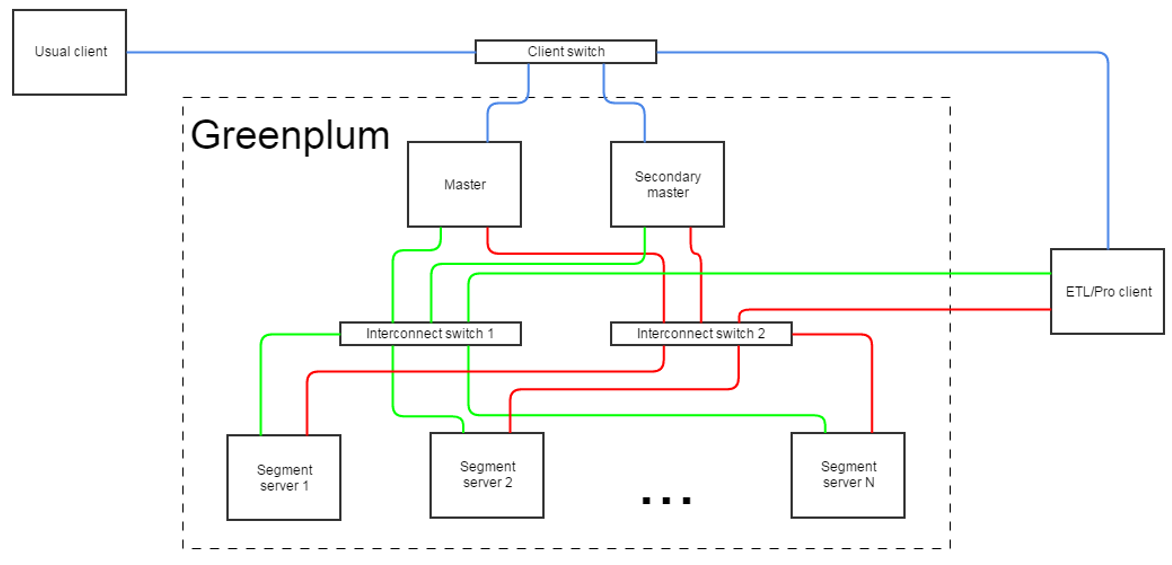
\includegraphics[width=100mm]{assets/distributed/Greenplum}
    \caption{Состав кластера и сетевое взаимодействие элементов Greenplum}
    \label{fig:Greenplum}
\end{figure}

При выборе числа серверов-сегментов важно правильно выбрать соотношение кластера «число процессоров/Тб данных» в
зависимости от планируемого профиля нагрузки на БД — чем больше процессорных ядер приходится на единицу данных, тем
быстрее кластер будет выполнять «тяжёлые» операции, а также работать со сжатыми таблицами.

При выборе числа сегментов в кластере (которое в общем случае к числу серверов никак не привязано) необходимо помнить
следующее \autocite{Greenplum}:
\begin{itemize}
    \item все ресурсы сервера делятся между всеми сегментами на сервере (нагрузкой зеркал, в случае если они располагаются на этих же серверах, можно условно пренебречь);
    \item каждый запрос на одном сегменте не может потреблять процессорных ресурсов больше, чем одно ядро CPU. Это означает, например, что, если кластер состоит из 32-ядерных серверов с 4-я сегментами GP на борту и используется в среднем для обработки 3-4 одновременных тяжёлых, хорошо утилизирующих CPU, запросов, «в среднем по больнице» CPU не будет утилизироваться оптимально. В данной ситуации лучше увеличить число сегментов на сервере до 6-8;
    \item штатный процесс бекапа и рестора данных «из коробки» работает только на кластерах, имеющих одинаковое число сегментов. Восстановить данные, забекапленные на кластере из 96 сегментов, в кластер из 100 сегментов без напильника будет невозможно.
\end{itemize}

В Greenplum реализуется классическая схема шардирования данных. Каждая таблица представляет из себя N+1 таблиц на всех
сегментах кластера, где N – число сегментов (+1 в этом случае — это таблица на мастере, данных в ней нет). На каждом
сегменте хранится 1/N строк таблицы. Логика разбиения таблицы на сегменты задаётся ключом (полем) дистрибуции – таким
полем, на основе данных которого любую строку можно отнести к одному из сегментов \autocite{Greenplum}.

По подробнее почитать про Greenplum можно в источнике. В данной главе приведена только краткая информация об общей
архитектуре и информация, относящаяся к тиражированию данных. \autocite{Greenplum}

\subsection{Бесконфликтные реплицированные типы данных}
\paragraph{Проблема репликации}
Предположим, реплики СУБД распределены по географическому признаку для ускорения работы приложения. А теперь пусть в разных репликах практически одновременно и независимо была изменена одна и та же строка. Какую строку считать правильно отражающей данные? Как восстановить согласованность между репликами? В общем случае, проблема одновременного обновления реплик не может быть разрешима. Поэтому большинство распределенных СУБД запрещают производить такие операции, например используя только один сервер для выполнения запросов. Однако существует некоторый класс структур данных, которые позволяют автоматически разрешать конфликты возникающие в процессе обновления нескольких реплик. Этот класс называется - бесконфликтные реплицированные типы данных или conflict-free replicated data types(CRDT). 
\paragraph{CRDT. Опеределение и виды}
CRDT обладают следующими характеристиками:
\begin{itemize}
    \item Приложение может обновлять реплики независимо, параллельно с другими репликами
    \item Алгоритм(как часть CRDT) автоматически разрешает возможные конфликты
    \item Данные в разных репликах могут быть в различных состояниях в один и тот же момент времени, но они гарантированно сойдутся спустя некоторое время 
\end{itemize}
Просто используя специализированные структуры данных было бы сложно добиться бесконфликтности, поэтому для ее достижения используются также специальные алгоритмы обновления данных. Алгоритмы определяют требования к структурам данных, а также могут накладывать дополнительные требования на сети передачи данных. Рассмотрим два основных вида алгоритмов:
\begin{itemize}
    \item Operation-based CRDTs. При обновлении данных, на реплике генерируется специальная функция обновления, которая затем рассылается всем другим нодам в сети. Каждая нода применяет эту функцию к своим данным и таким образом достигается консистентность. Важно, чтобы каждая функция была лишь раз применена на каждой ноде. Поэтому необходимо следить за тем, чтобы доставка гарантированно произошла и произошла только один раз. Связано это с тем, что функции могут быть коммутативными, но далеко не факт, что они будут идемпотентными(применение несколько раз подряд дает разные результаты).
    \item State-based CRDTs. При обновлении данных, репликам посылается полная локальная копия данных, после чего реплики локально у себя сливают эти изменения воедино, причем операция слияния (merge) обладает свойствами ассоциативности, коммутативности и идемпотентности, что позволяет уменьшить требования к каналам связи между репликами. 
    \item Delta-state CRDTs - оптимизированный вариант state-based CRDTs, когда посылаются только недавно примененные изменения вместо полной копии состояния.
\end{itemize}
Помимо алгоритмов, важную роль играют процессы сходимости между нодами. Для сходимости в случае Operation-based CRDTs, каждая нода обязана получить ровно одно сообщение с фукнцией обновления и для этого необходим надежный протокол доставки. В случае с State-base CRDTs, наличие коммутативного и идемпотентного оператора слияния позволяет утверждать, что данные постепенно сойдутся в любом случае, что дает нам право не беспокоиться о протоколе доставки. 
\paragraph{Примеры реализации}
На сегодняшний день известных CRDT не так много, одни из них: G-Counter (Grow only counter), PN-Counter (positive-negative counter), G-Set (grow only set) и несколько других типов. Основной особенностью всех этих типов данных является, то что каждая коллекция поддерживает узкий набор операций. А чтобы добавить например вычитание (некоммутативную операцию) в PN-Counter необходимо прибегать к хитрости и использовать два ворастающих счетчика типа G-Counter. Рассмотрим пример реалиции G-Counter-а. 
\begin{figure}[H]
    \centering
    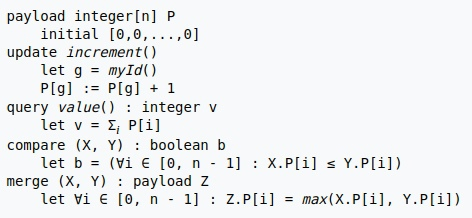
\includegraphics[width=100mm]{assets/distributed/G-Counter}
    \caption{Пример реализации Grow only Counter-а}
    \label{fig:G-Counter}
\end{figure}
Этот State-based счетчик сделан для кластера из n нод. Каждой ноде присвоен id, который можно получить вызвав функцию myid(). Таким образом, каждой ноде присваивается свой слот в массиве P, который нода может инкрементировать локально. Обновления расходятся по сети и при слиянии вычисляется максимум для каждого слота. При запросе значения счетчика все значения в слотах вектора суммируются и возвращаются в качестве ответа. Функция слияния является идемпотентной и коммутативной, поэтому данный счетчик является state-based.
Использование CRDT позволяет существенно упростить жизнь для разработчиков СУБД и облегчить работу с репликами. Уже сейчас CRDT используется во многих крупных проектах. В их число входит: Redis, Riak, Apple, Facebook. В дальнейшем использование CRDT будет только увеличиваться. 

\subsection{Интеграция БД и Internet}
\paragraph{Современные тенденции}
Заключаются в том, чтоб забыть о физических машинках и виртуалках, завернуть сервисы в контейнеры и перенести их в облако. Это позволяет разработчикам и компаниям быть более гибкими, 
упрощает разработку, тестирование и масштабирование приложений.

\subsubsection{Контейнеризация}
**Контейнеризация** обеспечивает ряд преимуществ, 
среди которых:

* **Изоляция:** Каждый контейнер представляет собой изолированную среду, 
что позволяет приложениям работать независимо друг от друга, 
не влияя на другие приложения или систему.
* **Портативность:** Контейнеры можно легко переносить между различными 
средами, будь то локальные машины, виртуальные машины или облачные платформы.
* **Масштабируемость:** Контейнеры можно легко масштабировать 
вверх или вниз в зависимости от потребностей приложения.
* **Эффективность:** Контейнеры используют меньше ресурсов, чем виртуальные машины, 
что делает их более экономичными.

\paragraph{Docker} ~\\

    Docker~--- средство виртуализации и менеджмента программ (сервисов), позволяющее гибко настраивать инфраструктуру проектов, и кратно облегчающее разработку, тестирование и масштабируемый деплой.
    Архитектура у Docker клиент-серверная, что означает наличие демона dockerd и клиентов docker, отправляющих демону команды (собери, скачай, запусти, пр.). Если вам нужно на коленке запустить оркестрацию
    (операции ``возьми n нод, запусти на них k заданий (образов Docker) и проследи, чтоб выполнились''), можно использовать docker swarm. \autocite{DockerSwarmConcepts} В проде такое лучше не использовать,
    потому что ноды приходится создавать ручками; иными словами, если у вас есть 2 машинки с разным количеством ресурсов каждая, придётся собственными силами подстраивать количество запускаемых на машинке нод,
    подстраиваясь под потребляемые ресурсы. Если требуется динамическое масштабирование, лучше посмотреть в сторону K8s.

    \textbf{Контейнеры} ~\\
    Основная идея~--- завернуть необходимый сервис (бинарники, скрипты, данные, конфиги) в легковесный \textbf{контейнер}, который далее будет запускаться на произвольном устройстве, способном запускать
    64-битный Linux (Windows и macOS под капотом запускают сначала виртуалку с Linux, и лишь на ней крутят Docker). Такой подход с упаковкой всего необходимого в контейнер позволяет не волноваться о том,
    что на хосте (устройство, где контейнер запущен) будет недоставать пакетов, возникнут проблемы с совместимостью и тому подобное.

    \textbf{Изолированность} ~\\
    Контейнеры из коробки являются изолированными сущностями~--- процессы, запущенные в одном контейнере не смогут влиять и даже смотреть на то, что запущенно в другом контейнере или на хосте, а для получения
    таковой функциональности придётся приложить дополнительные усилия. Также для каждого контейнера заводится свой сетевой стек.
    Обеспечивается такая изоляция средствами ядра Linux, а именно~--- \textbf{пространствами имён} (namespaces) и \textbf{контрольными группами} (control group). Первые отвечают за то, чтоб котнейнеры
    не подглядывали друг за другом; а вторые распределяют и ограничивают используемые контейнерами ресурсы хоста, гарантируют не только то, что контейнеры не будут голодать по памяти, CPU, дисковым операциям,
    но и то, что контейнеры не отберут все ресурсы у других потребителей.

    \textbf{Атаки на dockerd} ~\\
    Демон dockerd по умолчанию (можно запустить и в rootless режиме) требует root привилегий. Например, это требуется для пробрасывания директории хоста в контейнер. В связи с чем следует предоставлять
    управление демоном только тем пользователям, которым доверяешь. В пример можно привести атаку, в ходе которой корень файловой системы хоста примонтируется в директорию внутри контейнера, к которой
    у постороннего пользователя будет доступ. Для защиты от этого Docker использует не TCP сокеты, а UNIX сокеты, на которые можно поставить стандартные проверки прав доступа UNIX.
    Также существует атака с подменой образа. Например, подменить образ, который позднее будет загружен через \texttt{docker load} (локально) или \texttt{docker pull} (по сети), однако современные версии докера
    сверяют хэш-суммы образов, что сильно усложняет эксплуатацию уязвимости. \autocite{DockerSecurity} ~\\
    При использовании dockerd на устройстве рекомендуется все сервисы, запущенные на том же устройстве, тоже разнести по контейнерам.

    \textbf{Как можно доверять загружаемым образам} ~\\
    Часть Docker, позволяющая верифицировать целостность образов и их авторов путём проверки подписей называется Docker Content Trust (DCT). Сами образы при этом хранятся в \href{https://docs.docker.com/registry/}{Docker registry} (DockerHub~--- пример общедоступного registry).
    В репозитории (например ubuntu, mongo), где хранятся образы, создаётся набор ключей, которыми автор может подписывать по желанию теги этого репозитория, при это можно даже выпустить две версии одного тэга:
    подписанную и неподписанную. Пользователь репозитория может фильтровать теги доступные к загрузке~--- можно запретить использование неподписанных тегов. ~\\
    Доверие достигается следующим образом. У автора есть оффлайн-ключ (рутовый) и сертификат, с помощью которого создаются ключи и сертификаты тега (delegation keys) (обладание такими ключами позволяет вливать новые образы в репозиторий). \autocite{DockerSecurityTrust} У ползователя же на машинке лежит
    CA сертификат, которым подписан registry сертификат, а также собственный сертификат пользователя и ключ (последние нужны для того, чтоб registry мог верифицировать пользователя). \autocite{DockerSecurityCertificates}

    \textbf{PKI в docker swarm} ~\\
    Ноды в swarm'е используют TLS для аутентификации, авторизации и шифрования соединения с другими нодами. Когда созадётся управляющая нода (manager), она генерирует CA сертификат и ключевую пару для
    дальнейшего общения с остальными. Также генерируются два токена~--- для добавляемых в swarm нод-работников и нод-управляющих. Токен является комбинацией открытого ключа сертификата и секрета. Открытый ключ используется подключаемой нодой для валидации сертификата управляющей ноды, а секрет
    используется управляющей нодой для валидации подключаемой ноды. Далее управляющая выдаёт подключённой ноде новый сертификат, подписанный CA сертификатом. Таким образом устанавливается PKI, и далее ноды могут проверять, действительно ли с ними общаются разрешённые ноды. \autocite{DockerSwarmPKI}

    \textbf{Секреты в docker swarm} ~\\
    Когда в кластер добавляется секрет, он попадает в главную управляющую ноду с использованием TLS, далее реплицируется на остальные управляющие ноды, где хранится в зашифрованном логе Raft (используется для установления консенсуса между управляющими нодами, любознательные могут
    глянуть \href{http://thesecretlivesofdata.com/raft/}{анимацию}). Далее можно выдавать сервисам права на использование секретов, в таком случае секреты расшифровываются и монтируются в файловую систему контейнеров. Обновление/удаление/добавление секрета инициирует обновление сервиса,
    поэтому ротацию секретов придётся проводить в несколько шагов: добавить новый секрет, переключить сервис на его использование, удалить старый секрет. \autocite{DockerSwarmSecrets}

\paragraph{Kubernetes} ~\\
    Kubernetes~--- инструмент, умеющий запускать контейнеры на множестве хостов, следить за их состоянием, а также обновлять запущенные версии контейнеров, используя заданную политику (например, задача ``обнови реплики сервиса по очереди, переключая каждую из них лишь по завершении
    скриптов запуска и успешной проверки работоспособности''), откатывать сервис до одной из сохранённых версий. Но самое приятное~--- он умеет следить за количеством ресурсов на хостах и сам масштабирует сервис, понимая, можно ли добавить в него контейнер, или лучше удалить,
    чтоб остальные не голодали. Также K8s умеет производить обнаружение сервисов (хранить и выдавать при необходимости маршрут до сервиса), балансировку нагрузки, перезапуск контейнеров по триггеру, оркестрацию хранилищ, менеджмент секретов. В сравнении с Docker K8s более трудозатратно настраивается, но и возможностей у него побольше.
    Из явных отличий~--- уже упомянутые автомасштабирование и перезапуск сервисов в случае их выхода из строя. Да, можно и в swarm этого добиться, но зачем изобретать велосипед?

    \textbf{Из чего состоит} ~\\
    Сущность, получаемая после настройки K8s, называется кластером. Кластер состоит из набора нод-рабочих (worker node) (минимум одна на кластер), которые запускают у себя контейнеры. На этих нодах запускается поды (pods). Управляют всем отдельные ноды (control plane). В проде обычно запущено несколько управляющих нод для отказоустойчивости. \autocite{KuberComponents}

\subsubsection{Аутентификация и авторизация в Интернете}~\\

В распределенных системах регистрацией, идентификацией/аутентификацией занимается
сервис, реализующий СУБД. Приложения не имеют прямого доступа к данным
пользователя в БД, а обращаются к СУБД, которая возвращает данные, не позволяющие
скомпрометировать пользователя. Для решения таких задач существуют стандарты
идентификации. Самые распространенные из них это OAuth 2.0 \autocite{OAuth2.0}, OpenID Connect \autocite{OpenIDConnect}.~\\

С помощью OAuth 2.0 пользователь разрешает определенному сайту получить свои
закрытые данные из соцсетей, но без передачи сайту своих логинов / паролей. Например,
когда вы регистрируетесь на сайте через Facebook, то как раз и предоставляете этому сайту
разрешение получить из Facebook ваше имя, e-mail адрес и другие закрытые данные.~\\

Стандарт определяет следующие роли:

\begin{itemize}
    \item Resource Owner — пользователь, который заходит на Сайт и дает ему разрешение использовать свои закрытые данные из Соцсети.
    \item Client (он же Сайт) — приложение или интернет сайт, которым пользуется пользователь и которое взаимодействует с Authorization Server и Resource Server для получения закрытых данных пользователя.
    \item Authorization Server — сервер который проверяет логин/пароль пользователя, он же Соцсеть.
    \item Resource Server — хранит закрытую пользовательскую информацию, которую можно получить с помощью API. Authorization Server и Resource Server могут быть совмещены в одну систему.\autocite{OAuthRoles}
\end{itemize}

Теперь сам процесс. Детали конкретных реализаций могут различаться, но общая логика
будет всегда следующая:

\begin{itemize}
    \item Resource Owner заходит на Client, выбирает опцию “войти с помощью Соцсети”, сайт перенаправляет пользователя в Cоцсеть на Authorization Server.
    \item Authorization Server проверяет есть ли у пользователя активная сессия и, если нет, то показывает форму для логина.
    \item Resource Owner вводит свои логин/пароль и подтверждает, что определенные закрытые данные могут быть использованы Сайт, например имя пользователя или e-mail адрес.
    \item Authorization Server проверяет пользователя и перенаправляет на адрес Callback с результатом аутентификации и “Authorization Code”
    \item В ответ Client посылает “Authorization Code”, Client ID и Client Secret.
    \item Authorization Server проверяет присланные данные и формирует “access token” в формате JWT (JSON Web Token), подписанный своим приватным ключом. В этом же JWT может содержаться и “refresh token”, c помощью которого возможно восстановление сессии после ее окончания.
    \item После этого Client может запросить закрытую информацию пользователя с помощью вызова API, в который передается “access token”.
    \item Resource Server проверяет “access token” (например, используя открытый ключ Authorization Server) и предоставляет доступ к данным пользователя.\autocite{OAuthToken}
\end{itemize}

OpenID Connect является надстройкой над OAuth 2.0:

\begin{itemize}
    \item C помощью OAuth 2.0 выполняется только авторизация пользователя, т.е. о пользователе мы знаем только access token, с помощью которого можем получать определенные данные из Соцсети. Но access token ничего не говорит о личности пользователя и с помощью него мы не можем предоставить доступ к закрытым данным пользователя на нашем Сайте. OpenID Connect — добавляет сведения о логине и профиле пользователя (identity). Это как раз и позволяет реализовать его аутентификацию.
    \item OpenID Connect также добавляет возможность динамической регистрации и обнаружения сервисов “service discovery”. Это дает возможность строить системы SSO (Single Sign-On), в которых используется один логин для многих не связанных между собой сервисов.\autocite{OpenIDConnect}
\end{itemize}

OIDC расширяет OAuth 2.0 следующими основными возможностями:

\begin{itemize}
    \item Authorization Server, помимо access token и refresh token, возвращает “identity token” (ID Token). Он содержится в том же JWT. Из ID Token можно извлечь следующую информацию: имя пользователя, время входа в учетную запись, срок окончания действия ID Token. ID Token можно передавать между участниками.
    \item OIDC предоставляет дополнительное API, которые позволяет запрашивать информацию о пользователе и его текущих сессиях.\autocite{IDToken}
\end{itemize}

Диаграмма взаимодействия в OpenID Connect выглядит так же, как и в случае OAuth. Единственная разница заключается в содержимом запросов:

\begin{itemize}
    \item В первичном запросе на получение code добавляется дополнительный атрибут scope=openid.
    \item В результате работы алгоритма Client, помимо access и refresh token, получает ID Token.\autocite{IDToken}
\end{itemize}

\subsubsection{База Данных как SaaS (DBaaS)}
Что такое база данных как услуга (DBaaS)?

База данных как услуга (DataBase as a Service) - это управляемая сервисная услуга для облачных вычислений, 
предоставляющая доступ к базе данных без необходимости установки физического оборудования, установки программного обеспечения 
или настройки базы данных. Большинство задач по администрированию и обслуживанию базы данных берет на себя поставщик услуг, 
что позволяет пользователям быстро воспользоваться преимуществами сервиса базы данных.

В локальной вычислительной среде сервер баз данных является частью ИТ-инфраструктуры в центре обработки данных организации и устанавливается, 
управляется и обслуживается силами ИТ-отдела организации. Администратор базы данных отвечает за настройку и управление базами данных, 
запущенными на сервере.

В противоположность этому, в модели DBaaS поставщик обслуживает инфраструктуру системы и базу данных и предоставляет ее как полностью 
управляемый облачный сервис. Услуга включает в себя административные функции высокого уровня, такие как установка, настройка, обслуживание 
и обновление баз данных. Дополнительные задачи, такие как резервное копирование, исправление ошибок и управление производительностью, также 
обычно выполняются провайдером. Контроль над данными в базе данных остается в ведении клиента, а роль администратора заключается, прежде всего, в мониторинге использования базы данных,
управлении доступом пользователей и координации действий с поставщиком DBaaS по таким вопросам, как развертывание, исправление и обслуживание \autocite{DBaaS}. 

\paragraph{Преимущества DBaaS}

\begin{itemize}
\item **Снижение требований к управлению:** Поставщик DBaaS берет на себя многие рутинные обязанности по управлению и администрированию баз данных.
\item **Отказ от физической инфраструктуры:** Базовая ИТ-инфраструктура, необходимая для работы базы данных, предоставляется поставщиком DBaaS или поставщиком облачной платформы, на которой размещена среда DBaaS, если это разные компании.
\item **Экономия на оборудовании:** Поскольку инфраструктура системы больше не находится в помещении, клиентам не нужно инвестировать в серверы баз данных или планировать постоянную модернизацию оборудования.
\item **Дополнительная экономия средств:** Помимо снижения капитальных затрат, экономия может быть достигнута за счет уменьшения эксплуатационных расходов на электричество и охлаждение воздуха, сокращения площадей в центрах обработки данных, а также за счет возможного сокращения штата ИТ-специалистов.
\item **Большая гибкость и простота масштабирования:** Инфраструктура, поддерживающая базу данных, может быть гибко масштабирована по мере изменения использования базы данных, в отличие от более сложного и жесткого процесса, необходимого для масштабирования локальных систем.
\item **Быстрое развертывание базы данных:** DBaaS облегчает работу ИТ-специалистов организации, поскольку им не нужно заботиться о решении административных задач.
\item **Функции безопасности:** Поставщики облачных баз данных, как правило, имеют те или иные функции безопасности корпоративного уровня, такие как шифрование данных и контроль идентификации и доступа.
\end{itemize}

\paragraph{Недостатки DBaaS}

У DBaaS есть и потенциальные недостатки по сравнению с локальными базами данных. К потенциальным недостаткам DBaaS можно отнести следующее:

\begin{itemize}
\item **Отсутствие контроля над ИТ-инфраструктурой:** Это, как правило, самая существенная проблема при использовании DBaaS по сравнению с собственными решениями. При использовании управляемых баз данных ИТ-специалисты организации не имеют прямого доступа к серверам и устройствам хранения данных, на которых они работают. В результате они вынуждены полагаться на облачного провайдера для эффективного управления инфраструктурой.
\item **Зависимость от поставщика DBaaS:** Если у организации пропадет интернет-соединение или произойдет системный сбой у поставщика DBaaS, организация не сможет получить доступ к своей базе данных до тех пор, пока проблема не будет устранена.
\item **Безопасность:** В некоторых случаях это вызывает беспокойство, поскольку база данных контролируется поставщиком DBaaS, и организация не имеет прямого влияния на безопасность серверов, на которых хранятся ее базы данных. Согласно модели разделения ответственности за безопасность облачных сред, организации отвечают за некоторые аспекты безопасности данных и такие вещи, как управление идентификацией и доступом в средах DBaaS. Однако поставщик следит за безопасностью платформы баз данных и базовой инфраструктуры.
\item **Латентность:** Дополнительное время, необходимое для доступа к корпоративным данным через Интернет, может вызвать проблемы с производительностью. Эти проблемы возрастают при загрузке больших объемов данных, что, как правило, происходит медленно и занимает много времени.
\end{itemize}

\paragraph{Инструменты и вендоры DBaaS}

Среди инструментов DBaaS можно выделить следующие: \autocite{DBaaS}

\begin{itemize}
\item **Amazon DynamoDB:** полностью управляемый сервис баз данных NoSQL.
\item **Google Cloud SQL:** полностью управляемый сервис реляционных баз данных для MySQL, PostgreSQL и других баз данных SQL.
\item **Oracle Base Database Service:** реляционная система управления базами данных с добавленными возможностями мультимодельности.
\item **Azure SQL Database:** реляционная база данных SQL, использующая движок Microsoft SQL Server.
\item **SAP HANA Cloud:** гибридная реляционная/SQL база данных.
\item **MongoDB Atlas:** служба баз данных NoSQL.
\end{itemize}
	